%! TEX program = xelatex
\documentclass[font=Times]{gw-dissertation}[2021/11/19]
\usepackage[style=numeric-comp]{biblatex}  % a modern alternative to bibtex
\usepackage{floatrow}
\usepackage{booktabs} % table separation lines
\usepackage[section]{placeins} % limit floats (figs, tables, etc.) to the same sections
\usepackage[font={singlespacing, footnotesize}, labelfont=bf]{subcaption} % subfigures' captions
\usepackage{listings}
\usepackage{graphicx}
\usepackage[none]{hyphenat}  % disable hyphenation; not required by GW guideline
\usepackage{longtable}
\usepackage{lscape}
\usepackage{tikz} % visual computational graphs
\usepackage{tikzscale}
\usepackage{tikzit}
\usepackage{relsize}
\input{tikzit.tikzdefs}

% this style is applied by default to any tikzpicture included via \tikzfig
\tikzstyle{tikzfig}=[baseline=-0.25em,scale=0.5]

% these are dummy properties used by TikZiT, but ignored by LaTex
\pgfkeys{/tikz/tikzit fill/.initial=0}
\pgfkeys{/tikz/tikzit draw/.initial=0}
\pgfkeys{/tikz/tikzit shape/.initial=0}
\pgfkeys{/tikz/tikzit category/.initial=0}

% standard layers used in .tikz files
\pgfdeclarelayer{edgelayer}
\pgfdeclarelayer{nodelayer}
\pgfsetlayers{background,edgelayer,nodelayer,main}

% style for blank nodes
\tikzstyle{none}=[inner sep=0mm]

% include a .tikz file
\newcommand{\tikzfig}[1]{%
{\tikzstyle{every picture}=[tikzfig]
\IfFileExists{#1.tikz}
  {\input{#1.tikz}}
  {%
    \IfFileExists{./figures/#1.tikz}
      {\input{./figures/#1.tikz}}
      {\tikz[baseline=-0.5em]{\node[draw=red,font=\color{red},fill=red!10!white] {\textit{#1}};}}%
  }}%
}

% the same as \tikzfig, but in a {center} environment
\newcommand{\ctikzfig}[1]{%
\begin{center}\rm
  \tikzfig{#1}
\end{center}}

% fix strange self-loops, which are PGF/TikZ default
\tikzstyle{every loop}=[]


% this style is applied by default to any tikzpicture included via \tikzfig
\tikzstyle{tikzfig}=[baseline=-0.25em,scale=0.5]

% these are dummy properties used by TikZiT, but ignored by LaTex
\pgfkeys{/tikz/tikzit fill/.initial=0}
\pgfkeys{/tikz/tikzit draw/.initial=0}
\pgfkeys{/tikz/tikzit shape/.initial=0}
\pgfkeys{/tikz/tikzit category/.initial=0}

% standard layers used in .tikz files
\pgfdeclarelayer{edgelayer}
\pgfdeclarelayer{nodelayer}
\pgfsetlayers{background,edgelayer,nodelayer,main}

% style for blank nodes
\tikzstyle{none}=[inner sep=0mm]

% include a .tikz file
\newcommand{\tikzfig}[1]{%
{\tikzstyle{every picture}=[tikzfig]
\IfFileExists{#1.tikz}
  {\input{#1.tikz}}
  {%
    \IfFileExists{./figures/#1.tikz}
      {\input{./figures/#1.tikz}}
      {\tikz[baseline=-0.5em]{\node[draw=red,font=\color{red},fill=red!10!white] {\textit{#1}};}}%
  }}%
}

% the same as \tikzfig, but in a {center} environment
\newcommand{\ctikzfig}[1]{%
\begin{center}\rm
  \tikzfig{#1}
\end{center}}

% fix strange self-loops, which are PGF/TikZ default
\tikzstyle{every loop}=[]


% this style is applied by default to any tikzpicture included via \tikzfig
\tikzstyle{tikzfig}=[baseline=-0.25em,scale=0.5]

% these are dummy properties used by TikZiT, but ignored by LaTex
\pgfkeys{/tikz/tikzit fill/.initial=0}
\pgfkeys{/tikz/tikzit draw/.initial=0}
\pgfkeys{/tikz/tikzit shape/.initial=0}
\pgfkeys{/tikz/tikzit category/.initial=0}

% standard layers used in .tikz files
\pgfdeclarelayer{edgelayer}
\pgfdeclarelayer{nodelayer}
\pgfsetlayers{background,edgelayer,nodelayer,main}

% style for blank nodes
\tikzstyle{none}=[inner sep=0mm]

% include a .tikz file
\newcommand{\tikzfig}[1]{%
{\tikzstyle{every picture}=[tikzfig]
\IfFileExists{#1.tikz}
  {\input{#1.tikz}}
  {%
    \IfFileExists{./figures/#1.tikz}
      {\input{./figures/#1.tikz}}
      {\tikz[baseline=-0.5em]{\node[draw=red,font=\color{red},fill=red!10!white] {\textit{#1}};}}%
  }}%
}

% the same as \tikzfig, but in a {center} environment
\newcommand{\ctikzfig}[1]{%
\begin{center}\rm
  \tikzfig{#1}
\end{center}}

% fix strange self-loops, which are PGF/TikZ default
\tikzstyle{every loop}=[]


% bib file location; use only one single bib file
\addbibresource{reference.bib} 

% default figure search path
\graphicspath{{figs}}

% priority of the formats of figures
\DeclareGraphicsExtensions{.pdf,.png}

% load my own macros
%! TEX root = main.tex

% ISO-style vector notation
\RenewDocumentCommand{\vec}{m}{\symbfup{#1}}

% ISO-style matrix notation
\NewDocumentCommand{\mat}{m}{\symbfit{#1}}

% ISO-style upright ordinary differentiation
\NewDocumentCommand{\diff}{}{\mathop{}\!\symup{d}}

% helper for partial differential terms
\NewDocumentCommand{\pdiff}{mm}{\frac{\partial #1}{\partial #2}}

% vim:ft=tex


% frontmatter
%! TEX root = ../main.tex

% title of the thesis
\title{Feasibility Study of Physics-Informed Neural Network Modeling in Computational Fluid Dynamics}

% author name
\author{Pi-Yueh Chuang}

% ms degree
\prevdegree{B.S. in Power Mechanical Engineering, June 2008, National Tsing Hua University}
\prevdegree{M.S. in Mechanical Engineering, June 2012, National Taiwan University}

% date
\gradmonth{August}
\graddate{31}
\gradyear{2022}
\defdate{August 4th, 2022}

% advisor
\advisor{Lorena A. Barba}{Professor of Mechanical and Aerospace Engineering}

% school within GW
\school{School of Engineering and Applied Science}

% committee members (start from index 1 and continue the list)
\committee{Lorena A. Barba, Professor of Mechanical and Aerospace Engineering, Dissertation Director}
\committee{Michael W. Plesniak, Chair of the Department of Mechanical and Aerospace Engineering, Committee Member}
\committee{Elias Balaras, Professor of Mechanical and Aerospace Engineering, Committee Member}
\committee{Peng Wei, Assistant Professor of Mechanical and Aerospace Engineering, Committee Member}
\committee{Kyle Niemeyer, Associate Professor of Mechanical Engineering, Committee Member}
% vim:ft=tex

%! TEX root = ../main.tex
%\dedication{}
% vim:ft=tex

%! TEX root = ../main.tex
\acknowledgments{
I sincerely appreciate my wife, Chao-Yi.
My Ph.D. study is a long journey.
She has always been supportive and has never been impatient with my slow progress on this journey.
It is her who always told me to pursue what I like to do.

I have been appreciative of my advisor, Professor Lorena Barba.
She allowed me to explore any interests without worrying about anything.
She was always there to protect students no matter what troubles we encountered.

I am also grateful to all I have met at GW: Olivier, Tingyu, Naty, Gil, Anastasia, Paulina, Aditya, Akash, and so many other friends at GW.
We survived Covid-19 together, and we survived this long journey at GW together.

Finally, thanks to those reading this dissertation.
Thanks to everyone and everything in my life.
The current life is a result of all the events that happened in the past.
These events and all the people I met made me who I am right now.
}
% vim:ft=tex

%! TEX root = ../main.tex
\abstract{
Solving the Navier-Stokes equations with deep learning has been a popular research topic since the term {\it physics-informed neural networks} (PINNs) was coined by Raissi et al. in 2017.
A search on Google Scholar using "physics-informed neural networks" as the keyword revealed a rapid growth from 60 results in 2017 to 3,340 results in 2021.
Such a blooming in PINNs raised our interest in how ready PINNs are for computational fluid dynamics (CFD) applications in practical engineering.

This work aims to understand data-free PINNs' capability to solve CFD problems from the perspectives of predictability and controllability.
Predictability helps engineering practitioners estimate the cost for the desired accuracy level, and controllability means whether practitioners can control the cost and accuracy.
With the help of NVIDIA's Modulus---a Python tool set for PINNs, we conducted computational experiments to understand PINNs' numerical behaviors and limitations in solving the incompressible Navier-Stokes equations.

The computational experiments consist of two groups of benchmarks.
Benchmarks in the first group help us understand the following behaviors of PINNs when solving the incompressible Navier-Stokes equations:
\begin{enumerate*}[label=(\arabic*)]
    \item cost-performance ratios,
    \item convergence of errors with respect to model complexity of MLP (multilayer perceptron) networks, and
    \item weak and strong parallel scalability.
\end{enumerate*}
Further, we benchmarked several training strategies that have not been seen in PINNs' literature or have not been widely examined by other researchers.
These strategies include annealing loss aggregation, cyclical learning rate, stochastic weight averaging, and nonlinear conjugate-gradient methods.
We used the 2D Taylor-Green vortex at $Re=100$ for all benchmarks within this group.

In the second group of the benchmarks, we investigated PINNs' capability to solve flow problems with instabilities by conducting computational experiments with a 2D cylinder flow at $Re=200$.
In both physical experiments and conventional CFD simulations, such a flow eventually reaches an unsteady solution with periodic vortex shedding due to instability.
We wanted to understand PINNs' accuracy in predicting such unsteady solutions.
Benchmarks in this group used three types of PINNs:
\begin{enumerate*}[label=(\arabic*)]
    \item a steady data-free PINN,
    \item an unsteady data-free PINN, and
    \item an unsteady data-driven PINN trained against both the Navier-Stokes equations and simulation data from PetIBM.
\end{enumerate*}
In addition, we used a 2D cylinder flow at $Re=40$, which does not have instabilities, to validate the steady and unsteady data-free PINNs' capabilities in flow with immersed bodies.

Here we list the key findings from the first group of our benchmarks:
\begin{enumerate}[nolistsep]
    \item Under a given desired error level, the time cost of a PINN solver is several orders of magnitude slower than our in-house conventional CFD solver, PetIBM.
    For example, 20 seconds with PetIBM versus 2 hours with the PINN for an error level of $1e-3$.
    \item PINNs with the same training loss may give different prediction accuracies.
    This nondeterministic behavior grows when MLP networks' model complexity increases.
    We found that training losses may keep decreasing even when PDE residuals already stop improving.
    In such cases, only the residuals of initial conditions are improving, which does not help with prediction accuracy.
    This finding suggests that PDE residuals are better options for monitoring training progress.
    \item Errors decrease at a similar rate when we either increase the number of hidden layers by one or double the number of per-layer neurons in MLP networks.
    It suggests that the former is a better option to improve prediction accuracy than the latter because the former needs less computational cost.
    \item Unlike conventional numerical methods, PINNs' errors do not monotonically decrease when increasing MLP networks' degrees of freedom (DoFs).
    PINNs can have different accuracies under the same number of DoFs, indicating that DoFs are not a proper metric for PINNs' model complexity.
    \item The per-batch number of training points has a stronger effect on PINNs' time costs than the model complexity. However, the former has less influence than the latter on prediction accuracy.
    It suggests that increasing per-batch training points should come after increasing hidden layers or neurons when improving PINNs' accuracy.
    \item PINNs' weak scaling is above $90\%$ on average (with 1 to 8 GPUs), which helps scale per-batch training points on GPUs with limited memory space.
    \item If we defined workload using the number of training points, PINNs have strong-scaling efficiencies ranging from $91\%$ with 2 GPUs in the best case to $27\%$ with 8 GPUs in the worst case.
    \item Defining a proper quantitative metric to evaluate model complexity is necessary to study PINNs' convergence and scaling properties further.
    \item All new training strategies we tried did not have significant effects on improving time-to-solution and prediction accuracy.
\end{enumerate}

In the second group of our benchmarks, the validations of both the steady and unsteady data-free PINN solvers were successful against the 2D cylinder flow at $Re=40$.
PINNs' drag coefficients and surface pressure distribution were within the range of experimental data and conventional CFD simulations.

As for the 2D cylinder flow at $Re=200$, the unsteady data-free PINN solver could not predict vortex shedding within a simulation time of $t\in[0, 200]$.
The unsteady data-free PINN solver converged to a steady-state solution instead.
The data-driven PINN solver---trained against simulation results from PetIBM in $t \in [125, 140]$ and the Navier-Stokes equations in $t\in[125, 200]$---also converged to a steady-state solution when $t > 140$.
Moreover, the data-driven PINN solver failed to give meaningful predictions for $t<125$.
Nevertheless, all PINNs' drag coefficients agreed with conventional steady-state simulation results.

Besides the benchmarks, this work briefly introduces PINNs.
Starting from the difference between data-driven and data-free PINNs, we continue by introducing the history and the development of solving PDEs with data-free PINNs since 1994.
We discuss the open questions and known issues of data-free PINNs, which further motivated the present work.
In a later chapter, we detail the mathematical formulations related to PINNs.
Moreover, we compare PINNs to conventional numerical methods and show that PINNs is a special case of the least-square finite element methods.

We describe our in-house high-performance CFD code and associated verification and validation (V\&V) to compare conventional CFD methods and data-free PINNs.
The V\&V confirmed the correctness of our CFD code, and the subsequent performance benchmarks demonstrated its computational performance.
The in-house CFD code served as a baseline for PINNs' benchmarks.

In a nutshell, our results show that PINNs is a relatively new research area.
As we investigated the feasibility of PINNs, we found more open questions and challenges for PINNs to become an engineering tool.
While most studies in the literature focused on the theoretical capability of PINNs and toy PDEs, we hope our work can arouse others' interest in solving those challenges.
All the code, case configurations, scripts for pre-/post-processing, and definition files of containers are open and available online (https://github.com/piyueh/dissertation-repro-pack).
}
% vim:ft=tex

%! TEX root = ../main.tex
%\preface{}
% vim:ft=tex


% document body
\begin{document}

%! TEX root = main.tex
\nomenclature{$\odot$}{Hadamard product (element-wise multiplication)}
\nomenclature{$\otimes$}{Kronecker product}
\nomenclature{$N_l$}{Number of hidden layers in a fully-connected neural network}
\nomenclature{$N_n$}{Number of neurons per layer}
\nomenclature{$N_{bs}$}{Batch size during the training of a network}
\nomenclature{$\vec{x}$}{Spatial coordinate or spatial position vector (SI Unit: $\left(m, m\right)$)}
\nomenclature{$x$}{The first component in $\vec{x}$ (SI Unit: $m$)}
\nomenclature{$y$}{The second component in $\vec{x}$ (SI Unit: $m$)}
\nomenclature{$t$}{Time (SI Unit: $s$)}
\nomenclature{$\vec{u}$}{Velocity vector (SI Unit: $\left(\frac{m}{s}, \frac{m}{s}\right)$)}
\nomenclature{$u$}{The first component in $\vec{u}$ (SI Unit: $\frac{m}{s}$)}
\nomenclature{$v$}{The second component in $\vec{u}$ (SI Unit: $\frac{m}{s}$)}
\nomenclature{$p$}{Pressure field (SI Unit: $\frac{kg}{m\cdot s^2}$)}
\nomenclature{$lr$}{Learning rate}
\nomenclature{$\rho$}{Fluid density}
\nomenclature{$\nu$}{Kinematic viscosity (SI Unit: $\frac{m^2}{s}$)}
% vim:ft=tex


\chapter{Introduction}

    \section{Background and Motivation}
    %! TEX root = main.tex

If everyone only writes papers about bleeding edge methods, then each method will not have time to be sufficiently tested, analysed, and understood, especially that nowadays new methods come out every day.

Feasibility includes cost and performance (or more accurately, cost-performance ratio) and how controllable it is.
(Do not be confused with the performance here (i.e., accuracy) and the computational performance (wall time, more like a part of cost).)

Hardware and programming tools are the two vital resources for CFD (computational fluid dynamics) practitioners.
The boundaries of these resources have been pushed by deep learning in recent years.
For example, Google developed TPU (tensor processing unit), TensorFlow, and Colaboratory with deep learning in mind.
NVIDIA has been promoting its recent-generation GPUs (graphical processing units) for deep learning since 2015~\cite{Buck2015}.
Even supercomputing centers, such as those managed by the United States Department of Energy, shifted their focuses to deep learning for their next-generation hardware~\cite{USDepartmentofEnergy2019}.
As deep learning is leading the development of hardware and programming tools, it is inevitable to adopt deep learning in CFD one day.

CFD practitioners and researchers have been slowly catching up with this trend.
Nevertheless, most recent studies focus only on the proof-of-concept aspect of solving flow problems with deep neural networks.
They show different ways of incorporating neural networks in CFD, and they show that these new techniques are capable of giving visually acceptable results.
However, some critical questions regarding practical engineering remain unanswered in even the most recent studies.
From an engineering perspective, these questions are crucial during the planning and designing stage of a project.
For example:

\begin{itemize}
    \item In what types of numerical simulations, neural networks have advantages, in terms of time-cost and accuracy, over traditional CFD solvers?
    \item How does the hardware demand scale with problem sizes when using neural networks to solve flow problems?
    \item What is the time-cost of developing an in-house flow solver with neural network models?
    \item The trade-off between performance and accuracy is the key to CFD practice. How difficult or how easy is it to tune this balance when using neural network solvers?
\end{itemize}
    
The proposed works in this document will try to answer some of these questions. Section 1.3 gives a high-level description of our research aims, and section 3 gives the details of the planned tasks.

Recent advances in computing and programming techniques have motivated practitioners to revisit deep learning applications in computational fluid dynamics (CFD).
We use the verb "revisit" because deep learning applications in CFD already existed going back to at least the 1990s, for example, using neural networks as surrogate models \cite{Linse1993, Faller1997}.
Another example is the work of Lagaris and his/her colleagues \cite{lagaris_artificial_1998} on solving partial differential equations with fully-connected neural networks back in 1998.
Similar work with radial basis function networks can be found in reference \cite{Li2003}.
Nevertheless, deep learning applications in CFD did not get much attention until this decade, thanks to modern computing technology, including GPUs, cloud computing, high-level libraries like PyTorch and TensorFlow, and their Python APIs.

Solving partial differential equations with neural networks is particularly interesting to CFD researchers and practitioners.
The name physics-informed neural network (PINN) was coined by Raissi et al. \cite{raissi_physics-informed_2019} to describe such an application of deep learning.
These partial differential equations include the well-known Navier-Stokes equations—one of the Millennium Prize Problems.
The universal approximation theorem \cite{hornik_approximation_1991} implies that neural networks can model the solution to the Navier-Stokes equations with high fidelity and capture complicated flow details as long as networks are big enough.
This deep learning application is sometimes branded as unsupervised learning—it does not rely on human-provided data, making it sounds very *"AI."*
It is unsurprising to see headlines like *"AI has cracked the Navier-Stokes equations"* in recent popular science articles \cite{hao_ai_2020}.

The PINN method promises several advantages over traditional numerical methods (such as finite volume methods).
First, it is a mesh-free scheme.
A mesh-free scheme benefits engineering problems in which fluid flows interact with objects of complicated geometries.
Simulating these fluid flows with traditional numerical methods usually requires high-quality unstructured meshes.
Such meshes need time-consuming human intervention in the pre-processing stage before actual simulations.
The second benefit of PINN is that the trained models approximate the governing equations' general solutions, meaning there is no need to solve the equations repeatedly for different flow parameters.
For example, a flow model taking boundary velocity profiles as its input arguments can predict flows under different boundary velocity profiles after training.
Conventional numerical methods, on the contrary, require several simulations, with each one covering one boundary velocity profile.
This advantage helps in situations like engineering design optimization.
Traditionally, design optimization relies on sets of experiments to conduct parameter sweeps and find optimal parameters or geometries for products.

Given the stated benefits of PINN, enthusiasts have endeavored to show PINN's potential in real-world applications by reporting success stories of solving simple CFD problems with PINNs. 
However, despite the optimism shown in the literature, important information concerning the feasibility of PINN in practical applications is often missing from these success stories.
For example, few reports discuss the required computing resources, the computational performance, the convergence, or the error analysis of PINN.
PINN suffers from performance and solvability issues due to the need for high-order automatic differentiation and multi-objective nonlinear optimization.
For example, solving a second-order nonlinear differential equation requires at least three back-propagation passes for automatic differentiation (two for derivatives against model inputs and one for gradients against model parameters).
The training process needs to reduce all the residuals of differential equations, initial conditions, and boundary conditions.
Fluid flows are sensitive nonlinear dynamical systems in which a small change or error in inputs may produce a very different flow field.
So to get correct solutions, the optimization in PINN must minimize the loss to values extremely close to zero, further compromising the method's solvability and performance.

This paper provides our not-so-successful PINN story as a lesson learned to readers.
Our story includes two computational experiments as case studies to benchmark the PINN method's accuracy and computational performance.
The first case study, a Taylor-Green vortex, worked out, though not to our satisfaction.
We will discuss the performance of PINN using this case study.
The second case study, flow over a cylinder, did not even result in a physical solution.
We will discuss the frustration we encountered with PINN in this case study.

We built our PINN solver with the help of NVIDIA's Modulus library \cite{noauthor_modulus_nodate}.
Modulus is a high-level Python package built on top of PyTorch that helps users develop PINN-based differential equation solvers.
Also, in each case study, we also carried out simulations with our CFD solver, PetIBM \cite{chuang_petibm_2018}.
PetIBM is a traditional solver using staggered-grid finite difference methods with MPI parallelization and GPU computing.
PetIBM simulations in each case study served as baseline data.
All cases' configurations, post-processing scripts, and required Singularity image definitions can be found at reference \cite{pi_yueh_chuang_2022_6592457}.

This paper is structured as follows: the second section briefly describes the PINN method and an analogy to traditional CFD methods.
The third and fourth sections provide our computational experiments of the Taylor-Green vortex in 2D and a 2D laminar cylinder flow with vortex shedding.
Most discussions happen in the corresponding case studies.
The last section presents the conclusion and discussions that did not fit into either one of the cases.
% vim:ft=tex


    \section{Literature Review on Physics-Informed Neural Networks}
    %! TEX root = main.tex
\subsection*{Data-driven and data-free physics-informed neural networks (PINNs)}

To our knowledge, PINNs is an ambiguous term that has no authoritative definitions.
It is an umbrella term that includes all learning types that involve using PDEs in loss functions.

When Raissi et al. \cite{raissi_physics-informed_2017,raissi_physics_2017,raissi_physics-informed_2019} coined the term PINNs, they only distinguished two types of applications: {\it data-driven solutions of nonlinear partial differential equations} and {\it data-driven discovery of nonlinear partial differential equations}.
These two terms actually refer to forward and inverse problems.
In the same work, the term {\it data} in {\it data-driven} does not necessarily mean observed data (either experimental or computational).
For example, the test case of the Burger's equation in section 2.1 of \cite{raissi_physics-informed_2017} does not use any data from experiments or other numerical solvers.
The {\it data} in this example refers to the values of boundary conditions (BCs) and initial conditions (ICs) at selected collocation points.
As BCs and ICs are given and are part of PDEs' specification, from our viewpoint, these data do not carry the exactly same meaning as those in section \ref{sec:overview} in this thesis.
The mentioned example of Burger's equation in the work of Raissi et al. should be classified as a data-free approach per the description in section \ref{sec:overview}.

Under the classification in section \ref{sec:overview}, the work of Raissi et al. is actually a data-driven surrogate modeling with extra loss terms from governing PDEs.
Adding PDEs to the loss functions helps regulate or constrain the predictions of unseen data.
For example, if we have observed data at time $t_1$, $t_2$, $\cdots$, $t_{N_t}$ and spatial coordinates $\vec{x}_1$, $\vec{x}_2$, $\cdots$, $\vec{x}_{N_x}$, conventional data-driven approaches usually have inferior prediction accuracy for points not among these spatial-temporal coordinates.
Especially that because fluid flow is a sensitive and instable dynamical system, the predictions for $t < t_1$ and $t > t_{N_t}$ may deviate from the physics even qualitatively.
Adding PDEs to the training objectives helps in such situations.

In the remaining of this thesis, following the description in section \ref{sec:overview}, we will use {\it data-driven} to denote the use of experimental data or data generated by numerical solvers, and {\it data-free} refers situations when no experimental nor extra numerical data are involved. 

Raissi et al. did not distinguish the difference between {\it data-driven} and {\it data-free} as we do.
In PINNs, the treatment of observed data is the same to the treatment of Dirichlet BCs and ICs.
Under their PINNs, it is even possible to have no BCs and ICs.
One can just use observed data and governing PDEs to train the neural networks and build surrogate models.
Under this consideration, data-free PINNs in our terminology are just a special case of data-driven PINNs when no external data exists.
Hence, Raissi et al. used {\it data-driven} throughout their work, though some test cases are actually {\it data-free} in our classification.

When no observed data exist, and when BCs and ICs are used in training, the PINNs becomes the same as the one proposed by Dissanayake and Phan-Thien \cite{dissanayake_neural-network-based_1994}.
Moreover, the goal of PINNs is changed from constructing surrogate models to solving PDEs.
If the goal is to solve PDEs rather than just to create a surrogate model, most importantly, the BCs and ICs of PDEs do carry different meanings than observed data.
Observed data are allowed to and usually do have noise and fluctuations.
On the other hand, BCs and ICs are parts of PDEs, they should be met strictly.
So while we allow the model predictions to deviate from observations to some degree, we want the model predictions on both spatial and temporal boundaries to exactly match the BCs and ICs.
In terms of optimization, as we will discuss later, BCs and ICs are hard constraints, and observed data are simply objective.
Therefore, we believe it is necessary to exclude BCs and ICs from {\it data} and distinguish data-free and data-driven PINNs.

Most articles of PINNs in the recent years do not distinguish the two, either.
For example, references \cite{wang_understanding_2021,krishnapriyan_characterizing_2021,wang_when_2022} are about data-free PINNs and their capability in solving PDEs.
On the contrary, reference \cite{cai_physics-informed_2021} focuses on data-driven PINNs, and all test cases in this work are applications of data-driven PINNs.
While data-driven PINNs serve as methods for surrogate modeling, data-free PINNs are numerical methods for solving PDE/ODE solvers, meaning they are potential alternatives to mainstream CFD solvers, such as those using finite-difference, finite-volume, and finite-element methods.

In this work, we will focus on data-free PINNs.
Prior to the work of Raissi et al., there was no specific name for methods solving PDEs with neural network.
Therefore, in our work, we use data-free PINNs to refer to all methods of this type.

\subsection*{Literature review of data-free PINNs}

As mentioned previously, data-free PINNs can be traced back to at least 1994 \cite{dissanayake_neural-network-based_1994}.
In earlier studies, regardless of the networks' architectures, the derivatives of the model outputs with respect to model inputs were analytical.
It is the major reason that these studies could only use simple network architectures and smooth nonlinear activation functions. 
Activation functions are limited to those with smooth derivatives and simple expressions such as the sigmoid function.
For example, Dissanayake and Phan-Thien \cite{dissanayake_neural-network-based_1994} used MLP networks with 2-hidden layers, up to 10 neurons per layer, and the sigmoid function.
Lagaris' test cases \cite{lagaris_artificial_1998} were done with an MLP network with only one hidden layer and 10 neurons per layer.
Mai-Duy and Tran-Cong\cite{mai-duy_numerical_2001}, Li et al. \cite{li_numerical_2003}, Demirkaya et al. \cite{demirkaya_direct_2008}, and Wang et al. \cite{wang_meshless_2015} used RBF networks, which can be seen as a single-layer MLP network of RBF neurons and are easy to obtain the analytical derivatives.
McFall and his coworkers \cite{McFall2009,mcfall_solving_2010} used a single-layer MLP with up to 50 neurons.

We believe the limitation on the network architectures also limited the test cases used in these studies.
Among these earlier studies, only \cite{demirkaya_direct_2008,mcfall_solving_2010,wang_meshless_2015} showed applications to the Navier-Stokes equations for simple simulations (mostly 2D Poiseuille flow). 
Other works mentioned here tested their proposed methods with much simpler PDEs (e.g., 1D or 2D Poisson equations) and hinted the possibility of applications in flow problems.

More recently, automatic differentiation has been explicitly mentioned in literature, for example (\cite{berg_unified_2018,sirignano_dgm:_2018,dockhorn_discussion_2019,raissi_physics-informed_2017,raissi_physics-informed_2019,jin_nsfnets_2020,lu_deepxde:_2021,cai_physics-informed_2021}).
Using automatic differentiation makes it possible to approximate PDE solutions with more complicated neural network architectures.
Sirignano and Spiliopoulos \cite{sirignano_dgm:_2018} proposed an architecture similar to long short-term networks (LSTMs \cite{hochreiter_long_1997}).
Due to the recurrent nature of LSTMs, it is not practical, if not impossible, to obtain the analytical forms of the derivatives for this model either through manual derivation or computer symbolic derivations.
Studies that used MLP networks, on the other hand, were able to increase the complexity of the model by increasing the number of hidden layers and neurons.
Architectures with up to 10 hidden layers and 300 neurons per layer were used by the work of Jin et al. \cite{jin_nsfnets_2020}.

Another key component for data-free PINNs is the training process (a.k.a. model fitting).
The free parameters are determined through optimizing/minimizing the PDE residuals.
However, PDE solutions are bounded to ICs or/and BCs.
One can deem ICs and BCs as hard constraints when optimizing PDE residuals.
Earlier works of data-free PINNs converted this constrained problem to an unconstrained one by treating an approximate PDE solution as superposition of a nonhomogeneous-BC function and a solution under homogeneous BCs.
The nonhomogeneous-BC function is defined so that it meets the boundary conditions and initial conditions at collocation points on spatial-temporal boundaries.
The solution under homogeneous BCs, on the other hand, is further decoupled into the multiplication of a length function and a neural network.
The length function guarantees that the outputs of the neural network always diminish on Dirichlet boundaries and that the derivatives in normal directions always diminish on Neumann boundaries.
Lagaris \cite{lagaris_artificial_1998} showed an example of how to design such a length function and the nonhomogeneous-BC function for rectangular computational domains.
McFall and Mahan \cite{McFall2009} further proposed to use thin plane splines (TPSs) for both the nonhomogeneous-BC functions and the length functions in non-rectangular domains.
They further tested the proposed approach on the steady Navier-Stokes equations (steady boundary layer simulations and 2D Poiseuille flow). 
Note that TPSs are considered a type of RBFs, and one can classify the TPS method as an RBF neural network.
That says McFall and his coworkers' work can be extended to using other neural network architectures to model the length functions and nonhomogeneous-BC functions.
These studies, however, did not investigate applications in initial-boundary value problems.
Moreover, it has not been proved in theory nor extensively shown in experiments that claimed-to-be general length functions and nonhomogeneous-BC functions (like TPSs) can be applied to other PDEs and applications.
These functions may be problem-specific.

If we treat ICs and BCs as soft constraints, the training becomes a multi-objective optimization with each condition being an objective (i.e., a loss function).
A straightforward approach is to treat the residuals from BCs and ICs as losses and use weighted sum of all losses to obtain a single loss. 
An alternative viewpoint of the weighted sum of losses is to deem it as a special case of penalty function methods in constrained optimization.
The penalty functions are the residuals of ICs and BCs.
As other penalty method functions, this approach is considered to converge slower \cite{rudd_constrained_2014}.
However, most recent studies of PINNs (both data-free and data-driven) adopted this approach.
Using weighted sum of losses offers the simplicity in terms of mathematical expressions and programming.

Constant weights of one can be used in all terms in the weighted sum of losses (i.e., simply summing all losses), as seen in \cite{lagaris_artificial_1998,sirignano_dgm:_2018,dockhorn_discussion_2019}.
Though constant weights other than one can be used, no established guideline exists to assist in deciding proper values.
Jin et al. \cite{jin_nsfnets_2020} and Wang et al. \cite{wang_understanding_2021} proposed annealing loss algorithms to dynamically change the weight of each loss term during training.
These adaptive weights are determined using the magnitudes of losses' gradients with respect to model parameters.
It also involves the moving average of the weights from the current and previous iterations. 

To resolve the issues of problem-specific length and nonhomogeneous-BC functions in the first approach or the slow convergence in the second approach, Rudd and his coworkers \cite{rudd_constrained_2014,rudd_constrained_2015} solved the optimization problem in data-free PINNs with a constrained backpropagation method.
The hard constraints from BCs and ICs are satisfied during the training in this method.
This method, however, has not been widely tested and adopted by other researchers.

After converting to unconstrained problems, the actual optimization is usually done with methods based on gradient-descent and in a batched approach. 
Adam \cite{kingma_adam_2017} is the most popular optimizer nowadays in the literature of PINNs.
Nevertheless, Krishnapriyan et al. \cite{krishnapriyan_characterizing_2021} reported that L-BFGS performed significantly better than Adam for unknown reasons.
In \cite{jin_nsfnets_2020}, for example, Jin et al. also used L-BFGS to finalize the training.
However, even though L-BFGS needs much less computer memory than its origin, BFGS, it may still be impractical to use it in real-world problems due to the problem sizes.
And, to our knowledge, batch training is not well established for L-BFGS.
L-BFGS memorizes gradients from several past iterations.
So when the loss function's hypersurface changes at each iteration due to using different batches of data, the stored information of past gradients in L-BFGS may be problematic at the current iteration.

As for the nonlinear activation functions, to our best knowledge, it is still an unexplored area in data-free PINNs.
Most studies used either the sigmoid function or the hyperbolic tangent function without giving solid justifications.
Li et al. \cite{li_integration_2010} in 2010 proposed using wavelet functions for the activation.
However, their method has not received wide attention so far.
Moreover, no comparison or justification were given for why or how wavelet functions were better choices.
% vim:ft=tex

    \section{Research Aims}
    %! TEX root = main.tex

Data-free PINNs are still an ongoing research topic and pose many open questions.
Nevertheless, they hold several advantages over traditional numerical methods (such as finite-volume) that are attractive to CFD practitioners in practical engineering.
First, it is a mesh-free scheme.
A mesh-free scheme benefits engineering problems in which fluid flows interact with objects of complicated geometries.
Simulating these fluid flows with traditional numerical methods usually requires high-quality unstructured meshes.
Such meshes need time-consuming human intervention in the pre-processing stage before actual simulations.

The second benefit of data-free PINNs is that the trained models approximate the governing equations' general solutions, meaning there is no need to solve the equations repeatedly for different flow parameters.
For example, in tandem-cylinder flow simulations, if a neural network model also takes the distances between the cylinders as its inputs alongside spatial-temporal coordinates, the model can generate solutions for different distances after a single training session.
This feature benefits engineering optimization.
In the same tandem-cylinder example, the trained model can help determine the optimal distances and help heat transfer rates meet pre-defined specifications.
Conventional numerical methods, on the contrary, require several simulations (with each one covering one distance configuration) to find the optimal setting.

Data-free PINNs may be a potential solution to many engineering applications.
However, whether their current development is ready for practical engineering is doubtful.

Engineering solutions are always subject to some pre-defined specifications (e.g., minimum accuracy requirements) under certain constraints (e.g., time and monetary cost, existing tools, and resources).
To make a tool feasible for practical engineering, we believe two crucial factors are the predictability and controllability of the cost-performance relationship.
Predictably means engineers know how much cost is needed to get the desired performance.
Being controllable means engineers can further control the resulting performance by systematically changing costs.

We relate predictability and controllability to computational cost and accuracy for CFD applications.
Computational cost includes run times and required hardware.
For a given numerical method, the computational cost is affected by the degrees of freedom (DoFs) and the scalability of the method.
The convergence properties of the method dominate the cost-accuracy relationship.
With known convergence properties, given a preliminary result of some benchmark simulations on the target problem, engineers can predict how many extra degrees of freedom they need to lower the error level by a given amount, meaning the accuracy is controllable.
Additionally, with known scalability properties, engineers can determine what hardware resources and how much wall time they need.

However, to our best knowledge, these properties in data-free PINNs are still unclear and have not yet been investigated and reported in the literature.
Few reports studied either theoretically or experimentally the required computing resources, the computational performance, the convergence, or the error analysis of PINN.
Not to mention that even how to configure the network architectures and hyperparameters is still an open question. 

Since the earliest report of data-free PINNs in 1994, the configurations of neural network architectures have been some arbitrary choices based on the researchers' previous experience.
Even if one justifies the use of MLP networks with the universal approximation theory, the configurations of hyperparameters still seem to be arbitrary choices.
For example, Dissanayake and Phan-Thien acknowledged that their hyperparameter configurations were merely arbitrary choices.
Also, they did not notice a significant difference in the accuracies of different architecture configurations.
Dissanayake and Phan-Thien's report in 1994 may be outdated.
However, recently in 2019, Dockhorn \cite{dockhorn_discussion_2019} showed that data-free PINNs do not have clear properties in terms of convergence, run time, scalability, and being deterministic.

The model complexity of neural networks makes them difficult for theoretical analyses.
It may be the main reason the numerical properties of PINNs have not been widely studied.
On the other hand, PINNs suffer from performance and solvability issues due to the need for high-order automatic differentiation and constrained optimization.
The potentially high computational cost to solve PDEs with PINNs may block researchers from conducting studies through computational experiments.

In PINNs, automatic differentiation is a crucial component not only because it makes sophisticated models possible but also because it plays a vital role in computational cost.
Automatic differentiation is based on the chain rule of calculus, which backtracks each computing step that results in the current variable of interest.
Increasing the order of derivatives will at least double the computational graph.
So naively speaking, if the size of the computational graph from $x$ to $y$ is $N$, the size of the graph to evaluate $\frac{\partial^2 y}{\partial x^2}$ may be at least $4N$.
This is just a conservative estimation.
The actual graph size may be even higher due to many other factors.
So unlike regular data-driven deep learning applications (in which only first-order derivatives of model parameters are required), solving PDEs may demand much more hardware resources because of the high-order derivatives with respect to spatial-temporal coordinates.
Besides, the gradients with respect to model parameters will be one-order higher than the highest order of derivatives in PDEs. 
Even as recently as 2018, researchers \cite{sirignano_dgm:_2018} still used finite-difference to approximate derivatives of orders greater or equal to $2$.
However, as automatic differentiation is exact, using a finite-difference approximation to replace it might reduce the accuracy.

On the constrained optimization, when making BCs and ICs soft constraints (or using penalty function methods), the BCs and ICs are not guaranteed to be satisfied.
However, fluid flows are sensitive nonlinear dynamical systems in which a small change may produce a very different flow field.
How soft constraints and the errors in BCs and ICs affect the flow solutions have not been investigated.
Flow problems shown in the current literature of data-free PINNs are problems without known instability, for example, 2D Poiseuille flow, lid-driven cavity flow, or Taylor-Green vortex.
It is unclear if data-free PINNs can produce chaotic flow behaviors when instability plays a key role.

% vim:ft=tex


\chapter{PetIBM: a distributed-GPU incompressible Navier-Stokes solver}
%! TEX root = main.tex

Immersed-boundary methods solve fluid flow problems with the presence of solids by adding a body-force term to the Navier-Stokes equations.
This body-force term mimics the interface between fluid and solids.
Depending on the chosen formulations and schemes, the solids may be either rigid or deformable.
They can be stationary objects, objects moving under prescribed motions, or objects moving under feedback forces from fluid.
Different immersed-boundary methods may use different formulations for this body-force term to model the fluid-solid interfaces.

To be more precise, this forcing term models the force applied to the fluid by solids.
As this forcing term is part of the fluid governing equations defined in Eulerian coordinate systems, it is resolved on the same computational grid of the fluid, and solid-fluid interfaces are not anymore boundaries of the fluid's computational domain.
In other words, body-fitting meshes are unnecessary.
A benefit of such an approach is that a structured grid can be applied to solve flow problems with the presence of an object with complex geometry.

Consider a fluid problem with a fluid-solid interface.
$\Omega$ and $\Gamma$ corresponding to the whole domain of our interest and the fluid-solid interface.
The fluid-solid interface may be moving when viewing from a fixed coordinate system.
Given a time $t$ and a spatial coordinate $\vec{x}$ in an Eulerian coordinate system defined in $\Omega$, we can write the following Navier-Stokes equations for incompressible flow and the immersed-boundary projection method (IBPM):
\begin{subequations}\label{eq:mod-ns}
    \begin{align}[left=\empheqlbrace\,]
        &\pdiff{\vec{u}}{t} + \left(\vec{u} \cdot \nabla\right) \vec{u}
            =
            -\frac{1}{\rho}\nabla p + \frac{1}{Re} \nabla^2 \vec{u} + 
            \int\limits_{\Gamma} \vec{f}\left(\vec{\xi}\left(s, t \right), t\right) \delta\left(\vec{\xi}\left(s, t\right)-\vec{x}\right)\diff {\Gamma} 
            \label{eq:mod-ns-momentum} \\
        &\nabla \cdot \vec{u} = 0 \label{eq:mod-ns-cont}\\
        &\int\limits_{\Omega} \vec{u}\left(\vec{x}, t\right) \delta \left(\vec{x}-\vec{\xi}\left(s, t\right)\right)\diff\Omega
            =
            \vec{u}_{\Gamma}\left(s, t\right)
            \label{eq:mod-ns-body-vel}
    \end{align}
\end{subequations}

$\vec{u}$, $p$, $Re$, and $\rho$ are the velocity vector, pressure, Reynolds number, and fluid density, respectively.
$\vec{u}$ and $p$ are functions of $\vec{x}$ and $t$.
Though $\rho$ and viscosity can also be functions of $\vec{x}$ and $t$ for incompressible flow, we simply treat them as a constant in this work.
$s$ denotes the coordinate in a Lagrangian coordinate system defined on $\Gamma$.
For example, such a Lagrangian coordinate system is a curve in 2D problems, and a single scalar $s$ is enough to represent a coordinate on the interface.
$\vec{\xi}(s, t)$ is the coordinate in the Eulerian coordinate system that correspond to a Lagrangian coordinate $s$ on $\Gamma$ and at time $t$.
$\vec{u}_\Gamma$ represents the velocity of the fluid-solid interface.
Note $\vec{u}_\Gamma$ is a concept from the viewpoint of Lagrangian coordinate system.
$\vec{f}$ is the vector of force applied on fluid due to the presence of the fluid-solid interface.
It is defined in $\Omega$ and the Eulerian coordinate system, so it is a function of $\vec{x}$ and $t$.

$\delta$ is the Dirac delta function, i.e., $\delta(\vec{\xi}-\vec{x})$ equals to $1$ when $\vec{\xi} = \vec{x}$ and equals to $0$ otherwise.
With this Dirac delta function, the last term in \eqref{eq:mod-ns-momentum} is non-zero only at $\vec{x}$ that corresponds to the fluid-solid interface.
In other words, one can also write separate momentum equations without using the Dirac function:
\begin{equation}
\left\{
    \begin{array}{ll}
        \pdiff{\vec{u}}{t} + \left(\vec{u} \cdot \nabla\right) \vec{u}
            = -\frac{1}{\rho}\nabla p + \frac{1}{Re} \nabla^2 \vec{u}\text{,} & \vec{x} \notin \Gamma \\
        \pdiff{\vec{u}}{t} + \left(\vec{u} \cdot \nabla\right) \vec{u}
            = -\frac{1}{\rho}\nabla p + \frac{1}{Re} \nabla^2 \vec{u} + \vec{f}\left(\vec{x}, t \right)\text{,} & \vec{x} \in \Gamma \\
    \end{array}
\right. 
\end{equation}
It's clear now that only $\vec{x}$ exactly on fluid-solid interfaces is under the influence of the added body force.

The same logic applies to \eqref{eq:mod-ns-body-vel}.
In continuous space, equation \eqref{eq:mod-ns-body-vel} simply means $\vec{u}\left(\vec{x}, t\right)=\vec{u}_\Gamma\left(s, t\right)$ for $\vec{x} \in \Gamma$ and when $\vec{x}=\vec{\xi}\left(s, t\right)$.
It means the flow velocity on $\Gamma$ must satisfy the no-slip condition.
As $\Gamma$ is not a boundary of $\Omega$, this no-slip condition can not be specified as a boundary condition and hence is included in \eqref{eq:mod-ns}.

Though the integrals in the last term of \eqref{eq:mod-ns-momentum} and \eqref{eq:mod-ns-body-vel} seem unnecessary, having the integral or not makes difference when applying discretization in numerical methods.
Because we are not using body-fitting mesh, and the fluid-solid interface is arbitrary, it is almost impossible to have computational nodes located exactly on $\Gamma$.
Hence, to capture the effect of the interface, the delta function needs to be relaxed, i.e., $\delta \ne 0$ for $\lVert \vec{\xi}-\vec{x} \rVert$ smaller than a certain predefined tolerance.
Or, it can be made to some smooth function that approaches to zero when $\lVert \vec{\xi}-\vec{x} \rVert$ approaches infinity.
This kind of delta function is called regularized Dirac delta function.
And using a regularized delta function makes the fluid-solid interface duffuse: if we plot the integral in the last term of equation \eqref{eq:mod-ns-momentum} on a discretized 2D Cartesian grid of $\Omega$, the $\Gamma$ will look like a band, rather than a curve.

In PetIBM, we use the following regularized Dirac function:
\begin{equation}\label{eq:regularized-dirac}
    \delta\left(r\right)=\left\{
        \begin{array}{ll}
            \frac{1}{6 \Delta r}\left[
                5-3 \frac{r}{\Delta r}-\sqrt{-3\left(1-\frac{r}{\Delta r}\right)^{2}+1}
            \right] & \text { for } 0.5 \Delta r \le r \le 1.5 \Delta r \\
            \frac{1}{3 \Delta r}\left[
                1+\sqrt{-3\left(\frac{r}{\Delta r}\right)^{2}+1}
            \right] & \text { for }r \le 0.5 \Delta r \\
            0 & \text { otherwise }
        \end{array}
    \right.
\end{equation}
where $r \equiv \lVert\vec{\xi}-\vec{x}\rVert_2$, and $\Delta r$ is a user-provided parameter to determine the effective range of the regularized Dirac function.

The next step is to discretize the governing equations.
The IBPM is based on the following block-matrix system that can be generated from most discretization and time marching schemes:
\begin{equation}\label{eq:block-sys-ns}
    \begin{bmatrix}
        A & G & H \\
        D & 0 & 0 \\
        E & 0 & 0
    \end{bmatrix}
    \begin{bmatrix}
        \vec{u}^{n+1} \\
        \vec{p}^{n+1} \\
        \vec{f}^{n+1}
    \end{bmatrix}
    =
    \begin{bmatrix}
        \vec{\gamma}^n \\
        0 \\
        \vec{u}_\Gamma^{n+1}
    \end{bmatrix}
    +
    \begin{bmatrix}
        \vec{bc}_1 \\
        \vec{bc}_2 \\
        0
    \end{bmatrix}
\end{equation}
where $A$, $G$, and $D$ correspond to the $\frac{1}{\Delta t}I+\alpha\frac{1}{Re}L$, gradient, and divergence operators of a given spatial discretization. 
$L$ is the Laplacian operator, and $alpha$ is a coefficient that depends on chosen time marching scheme for the diffusion term.
$H$ and $E$ are the operator from substituting equation \eqref{eq:regularized-dirac} into equation \eqref{eq:mod-ns} and the discretizing the forcing terms and \eqref{eq:mod-ns-body-vel}.
Note that only matrix $A$ is a square matrix, while others are not.
Superscript $n+1$ and $n$ denote the $n+1$-th and $n$-th time steps.
$\vec{\gamma}^n$ represents the results of explicit terms from the selected time marching schemes.
Though having a superscript $n$, $\vec{\gamma}^n$ can actually depend on solutions from $n-1$, $n-2$, and so on, depending on the schemes.
$\vec{bc}+1$ and $\vec{bc}_2$ are the artifacts that generated from eliminating BCs from operators.

Reference \cite{taira_immersed_2007} shows an example of how these operators are actually defined using staggered Cartesian grid for spatial discretization, Adams-Bashforth for marching the convection term, and Crank-Nicolson for marching the diffusion term can be found in \cite{taira_immersed_2007}.
Here we will continue on assuming we already have these operators to save space, and we can focus on the solution scheme of this block matrix system using the decoupled IBPM of reference \cite{li_efficient_2016}.

Equation \ref{eq:block-sys-ns} is indefinite and difficult to solve.
To solve such a system, in decoupled IBPM, we define the following composite matrices and composite vectors: 
\begin{equation}\label{eq:composites}
    \begin{gathered}
        \bar{A} \equiv \begin{bmatrix} A & H \\ E & 0 \end{bmatrix};\
        \bar{G} \equiv \begin{bmatrix} G \\ 0 \end{bmatrix};\
        \bar{D} \equiv \begin{bmatrix} D & 0 \end{bmatrix}
        \\
        \vec{q}^{n+1} \equiv \begin{bmatrix} \vec{u}^{n+1} \\ \vec{f}^{n+1} \end{bmatrix};\
        \bar{\vec{\gamma}}_1 \equiv \begin{bmatrix} \vec{\gamma}^n + \vec{bc}_1 \\ \vec{u}_\Gamma^{n+1}\end{bmatrix};\
        \bar{\vec{\gamma}}_2 \equiv \vec{bc}_2
    \end{gathered}
\end{equation}
The original block system in \eqref{eq:block-sys-ns} can be re-arranged to:
\begin{equation}
    \begin{bmatrix}
        \bar{A} & \bar{G} \\
        \bar{D} & 0
    \end{bmatrix}
    \begin{bmatrix}
        \vec{q}^{n+1} \\
        \vec{p}^{n+1}
    \end{bmatrix}
    =
    \begin{bmatrix}
        \bar{\vec{\gamma}}_1 \\
        \bar{\vec{\gamma}}_2
    \end{bmatrix}
\end{equation}

The next step is to apply two successive block-LU decompositions.
The first block-LU decomposition decouples the pressure field from the new unknown $\vec{q}^{n+1}$:
\begin{equation}
    \begin{bmatrix}
        \bar{A} & 0 \\
        \bar{D} & -\bar{D}\bar{A}^{-1}\bar{G}
    \end{bmatrix}
    \begin{bmatrix}
        I & \bar{A}^{-1}\bar{G} \\
        0 & I
    \end{bmatrix}
    \begin{bmatrix}
        \vec{q}^{n+1} \\
        \vec{p}^{n+1}
    \end{bmatrix}
    =
    \begin{bmatrix}
        \bar{A} & 0 \\
        \bar{D} & -\bar{D}\bar{A}^{-1}\bar{G}
    \end{bmatrix}
    \begin{bmatrix}
        \vec{q}^* \\
        \vec{p}^{n+1}
    \end{bmatrix}
    =
    \begin{bmatrix}
        \bar{\vec{\gamma}}_1 \\
        \bar{\vec{\gamma}}_2
    \end{bmatrix}
\end{equation}
which leads to the following sequence of operations:
\begin{subequations}
    \begin{align}
        & \bar{A} \vec{q}^* = \bar{\vec{\gamma}}_1\label{eq:dibpm-lu1-1} \\
        & \bar{D}\bar{A}^{-1}\bar{G} \vec{p}^{n+1} = \bar{D} \vec{q}^* - \bar{\vec{\gamma}}_2\label{eq:dibpm-lu1-2} \\
        & \vec{q}^{n+1} = \vec{q}^* - \bar{A}^{-1}\bar{G} \vec{p}^{n+1}\label{eq:dibpm-lu1-3}
    \end{align}
\end{subequations}
Noticing the zero submatrices in $\bar{G}$ and $\bar{D}$, we can split equations \eqref{eq:dibpm-lu1-2} and \eqref{eq:dibpm-lu1-3} to:
\begin{subequations}
    \begin{align}
        & D\bar{A}_{00}^{-1}G \vec{p}^{n+1} = D \vec{u} - \vec{bc}_2\label{eq:dibpm-lu1-4} \\
        & \vec{u}^{n+1} = \vec{u}^* - \bar{A}_{00}^{-1}G \vec{p}^{n+1}\label{eq:dibpm-lu1-5} \\
        & \vec{f}^{n+1} = \vec{f}^* - \bar{A}_{10}^{-1}G \vec{p}^{n+1}\label{eq:dibpm-lu1-6}
    \end{align}
\end{subequations}
where $\bar{A}_{00}^{-1}$ and $\bar{A}_{10}^{-1}$ are the upper-left and lower-left submatrices in $\bar{A}^{-1}$.
The composite operator $\bar{A}$ is still indefinite, and step \eqref{eq:dibpm-lu1-1} is also tough to solve directly.
Therefore, a second block-LU decomposition is applied to solve $\vec{q}^{*}$ in \eqref{eq:dibpm-lu1-1}:
\begin{equation}
    \begin{bmatrix}
        A & 0 \\
        E & -EA^{-1}H
    \end{bmatrix}
    \begin{bmatrix}
        I & A^{-1}H \\
        0 & I
    \end{bmatrix}
    \begin{bmatrix}
        \vec{u}^* \\
        \vec{f}^*
    \end{bmatrix}
    =
    \begin{bmatrix}
        A & 0 \\
        E & -EA^{-1}H
    \end{bmatrix}
    \begin{bmatrix}
        \vec{u}^{* *} \\
        \vec{f}^*
    \end{bmatrix}
    =
    \begin{bmatrix}
        \vec{\gamma}^n + \vec{bc}_1 \\
        \vec{u}_\Gamma^{n+1}
    \end{bmatrix}
\end{equation}
and we end up with the following sequence:
\begin{subequations}
    \begin{align}
        & A u^{* *} = \vec{\gamma}^n + \vec{bc}_1\label{eq:dibpm-lu2-1} \\
        & EA^{-1}H \vec{f}^* = E \vec{u}^{* *} - \vec{u}_\Gamma^{n+1}\label{eq:dibpm-lu2-2} \\
        & \vec{u}^* = \vec{u}^{* *} - A^{-1}H \vec{f}^*\label{eq:dibpm-lu2-3}
    \end{align}
\end{subequations}
The order of solving is then:
\begin{subequations}
    \begin{align}
        & A u^{* *} = \vec{\gamma}^n + \vec{bc}_1\label{eq:dibpm-order1-1} \\
        & EA^{-1}H \vec{f}^* = E \vec{u}^{* *} - \vec{u}_\Gamma^{n+1}\label{eq:dibpm-order1-2} \\
        & \vec{u}^* = \vec{u}^{* *} - A^{-1}H \vec{f}^*\label{eq:dibpm-order1-3}\\
        & D\bar{A}_{00}^{-1}G \vec{p}^{n+1} = D \vec{u}^* - \vec{bc}_2\label{eq:dibpm-order1-4} \\
        & \vec{u}^{n+1} = \vec{u}^* - \bar{A}_{00}^{-1}G \vec{p}^{n+1}\label{eq:dibpm-order1-5} \\
        & \vec{f}^{n+1} = \vec{f}^* - \bar{A}_{10}^{-1}G \vec{p}^{n+1}\label{eq:dibpm-order1-6}
    \end{align}
\end{subequations}

Note that because $A$ has a format of $\frac{1}{\Delta t}I + \alpha \frac{1}{Re}L$, the Talyor series expansion of $A^{-1}$ is
\begin{equation}\label{eq:approx-A-inv}
    A^{-1} = \Delta t \sum\limits_{i=0}^{\infty} \left(-1\right)^{n}\left(\frac{\alpha\Delta t}{Re}\right)^n L^n
\end{equation}
And similarly, we can reformat $\bar{A}$ to a structure of $\frac{1}{\Delta t}I + S$ so that the inverse of $\bar{A}$ has a Taylor series expansion of
\begin{equation}\label{eq:approx-A-bar-inv}
    \bar{A}^{-1} = \Delta t \sum\limits_{i=0}^{\infty}\left(-1\right)^{n}\Delta t^n S^n
\end{equation}
where
\begin{equation}
    S = \begin{bmatrix}
        \frac{\alpha \Delta t}{Re}L & H \\
        E & -\frac{1}{\Delta t}I
    \end{bmatrix}
\end{equation}

In order to speed up the solving process, in the solution workflow, we can replace $A^{-1}$ and $\bar{A}^{-1}$ with truncated Taylor series expansions.
The most common approach is to use only the first-order approximation, i.e., use only the first term in the series expansions.
That is, $A^{-1} \approx \Delta t I$ and $\bar{A}^{-1} \approx \Delta t I$, where $I$ denotes the identity matrix with a corresponding dimension. ($A$ and $\bar{A}$ have different dimensions.)
Further, under the first-order approximation, the submatrices $\bar{A}_{00}^{-1}$ and $\bar{A}_{10}^{-1}$ can be found to be $\Delta t I$ and $0$.

The following is the actual solution workflow under the first-order approximation:
\begin{subequations}\label{eq:dibpm-first-order}
    \begin{align}
        & A u^{* *} = \vec{\gamma}^n + \vec{bc}_1\label{eq:dibpm-order2-1} \\
        & \Delta t EH \vec{f}^{n+1} = E \vec{u}^{* *} - \vec{u}_\Gamma^{n+1}\label{eq:dibpm-order2-2} \\
        & \vec{u}^* = \vec{u}^{* *} - \Delta t H \vec{f}^{n+1}\label{eq:dibpm-order2-3}\\
        & \Delta t DG \vec{p}^{n+1} = D \vec{u}^* - \vec{bc}_2\label{eq:dibpm-order2-4} \\
        & \vec{u}^{n+1} = \vec{u}^* - \Delta t G \vec{p}^{n+1}\label{eq:dibpm-order2-5}
    \end{align}
\end{subequations}

Using higher-order approximations for $A^{-1}$ and $\bar{A}^{-1}$ is achievable through the Taylor series expansions in \eqref{eq:approx-A-inv} and \eqref{eq:approx-A-bar-inv}.
However, the resulting linear systems in \eqref{eq:dibpm-order1-2} and \eqref{eq:dibpm-order1-4} may not be sparse due to the exponential terms in the Taylor series expansions.

In this section, we only described the specific solver (decoupled IBPM) we used to create the baseline data for benchmarking PINNs.
For other available solvers in PetIBM, please refer to the documentation in \cite{chuang_petibm:_2018}.
% vim:ft=tex

    \section{Mathematical Formulation}
    %! TEX root = main.tex
PetIBM solves the Navier-Stokes equations on an extended discretization grid that includes the interior of the immersed boundary.
To model the presence of the boundary, a forcing term is added to the momentum equation and an additional equation for the no-slip condition completes the system.
Variants of the immersed-boundary method (IBM) depend on how one models the forcing.
In PetIBM, we use regularized-delta functions to transfer data between the Eulerian grid and the Lagrangian boundary points.
The system of equations is:

\begin{equation}
\begin{cases}
\frac{\partial \symbf{u}}{\partial t} + \symbf{u} \cdot \nabla \symbf{u} = -\nabla p + \frac{1}{Re} \nabla^2 \symbf{u} + \int_{s}{\symbf{f} \left( \symbf{\xi} \left( \symit{s}, \symit{t} \right) \right) \delta \left( \symbf{\xi} - \symbf{x} \right)} d\symit{s} \\
\nabla \cdot \symbf{u} = 0 \\
\symbf{u} \left( \symbf{\xi} \left( \symit{s}, t \right) \right) = \int_{\symbf{x}}{\symbf{u} \left( \symbf{x} \right)} \delta \left( \symbf{x} - \symbf{\xi} \right) d\symbf{x}
\end{cases}
\end{equation}

where $\symbf{u}$ is the velocity field, $p$ is the fluid pressure, and $Re$ is the Reynolds number.

Currently, PetIBM provides two application codes implementing different versions of the IBM: (1) an immersed-boundary projection method (IBPM) based on the work of \cite{taira_colonius_2007} and (2) a decoupled version of the IBPM proposed by \cite{li_et_al_2016}.
Those two methods fit into the framework of the projection approach of \cite{perot_1993}.
The equations are fully discretized (space and time) to form an algebraic system to be solved for the velocity $u^{n+1}$, the pressure field $\phi$, and the Lagrangian forces $\tilde{f}$.
The discretized system is:

\begin{equation}
\left[
\begin{matrix}
A & G & H \\
D & 0 & 0 \\
E & 0 & 0
\end{matrix}
\right]
\left(
\begin{matrix}
u^{n+1} \\
\phi \\
\tilde{f}
\end{matrix}
\right)
=
\left(
\begin{matrix}
r^n \\
0 \\
u_B^{n+1}
\end{matrix}
\right)
+
\left(
\begin{matrix}
bc_1 \\
bc_2 \\
0
\end{matrix}
\right)
\end{equation}

where $D$, $G$, and $A$ are the divergence, gradient, and implicit operators, respectively.
$E$ and $H$ are the interpolation and spreading operators, respectively, used to transfer the data between the Eulerian grid and the Lagrangian boundary points.
On the right-hand side, $r^n$ gathers all the explicit terms and $u_B^{n+1}$ is the known (prescribed) boundary velocity; $bc_1$ and $bc_2$ contain the boundary terms that arise from the discretization of momentum and continuity equations, respectively.

In the IBPM, we solve a modified Poisson system for the pressure field and Lagrangian forces, coupled together.
This way, the divergence-free condition and no-slip constraint are simultaneously enforced on the velocity field at the end of the time step.
The fully discretized system can be cast into the following:

\begin{equation}
\left[
\begin{matrix}
A & Q_2 \\
Q_1 & 0
\end{matrix}
\right]
\left(
\begin{matrix}
u^{n+1} \\
\lambda
\end{matrix}
\right)
=
\left(
\begin{matrix}
r_1 \\
r_2
\end{matrix}
\right)
\end{equation}

with

\begin{equation*}
Q_1 \equiv \left[ \begin{matrix} D \\ E \end{matrix} \right] ;\
Q_2 \equiv \left[ G, H \right] ;\
\lambda \equiv \left( \begin{matrix} \phi \\ \tilde{f} \end{matrix} \right) ;\
r_1 \equiv r^n + bc_1 ;\
r_2 \equiv \left( \begin{matrix} bc_2 \\ u_B^{n+1} \end{matrix} \right)
\end{equation*}

In practice, we never form the full system.
Instead, we apply a block-LU decomposition as follows:

\begin{equation}
\left[
\begin{matrix}
A & 0 \\
Q_1 & -Q_1A^{-1}Q_2
\end{matrix}
\right]
\left[
\begin{matrix}
I & A^{-1}Q_2 \\
0 & I
\end{matrix}
\right]
\left(
\begin{matrix}
u^{n+1} \\
\lambda
\end{matrix}
\right)
=
\left[
\begin{matrix}
A & 0 \\
Q_1 & -Q_1A^{-1}Q_2
\end{matrix}
\right]
\left(
\begin{matrix}
u^* \\
\lambda
\end{matrix}
\right)
=
\left(
\begin{matrix}
r_1 \\
r_2
\end{matrix}
\right)
\end{equation}

Thus, we retrieve the sequence of operations of the traditional projection method.
We solve a system for an intermediate velocity field that is corrected, after solving a modified Poisson system for the variable $\lambda$, to enforce the divergence-free condition and the no-slip constraint at the location of the immersed boundary.
The sequence is:

\begin{align}
& A u^* = r_1 \\
& Q_1A^{-1}Q_2 \lambda = Q_1 u^* - r_2 \\
& u^{n+1} = u^* - A^{-1}Q_1 \lambda
\end{align}

The IBPM implemented in PetIBM solves, at every time step, Equations (5) to (6).
(Note: the inverse of the implicit operator $A^{-1}$ is approximated by a finite Taylor series expansion.)


The IBPM requires solving, at each time step, an expensive modified Poisson system, $Q_1A^{-1}Q_2$, whose non-zero structure changes when the location of the immersed boundary is moving.
In the PetIBM implementation of the decoupled IBPM, we apply a second block-LU decomposition to decouple the pressure field from the Lagrangian forces and recover a classical Poisson system.
The fully discretized algebraic system can be cast into:

\begin{equation}
\left[
\begin{matrix}
A & H & G \\
E & 0 & 0 \\
D & 0 & 0
\end{matrix}
\right]
\left(
\begin{matrix}
u^{n+1} \\
\tilde{f} \\
\phi
\end{matrix}
\right)
=
\left(
\begin{matrix}
r^n \\
u_B^{n+1} \\
0
\end{matrix}
\right)
+
\left(
\begin{matrix}
bc_1 \\
0 \\
bc_2
\end{matrix}
\right)
\end{equation}

The velocity $u^{n+1}$ and the Lagrangian forces $\tilde{f}$ are coupled together to form a new unknown $\gamma^{n+1}$, as follows:

\begin{equation}
\left[
\begin{matrix}
\bar{A} & \bar{G} \\
\bar{D} & 0
\end{matrix}
\right]
\left(
\begin{matrix}
\gamma^{n+1} \\
\phi
\end{matrix}
\right)
=
\left(
\begin{matrix}
\bar{r_1} \\
\bar{r_2}
\end{matrix}
\right)
\end{equation}

where

\begin{equation*}
\bar{A} \equiv \left[ \begin{matrix} A & H \\ E & 0 \end{matrix} \right] ;\
\bar{G} \equiv \left[ \begin{matrix} G \\ 0 \end{matrix} \right] ;\
\bar{D} \equiv \left[ \begin{matrix} D & 0 \end{matrix} \right]
\end{equation*}

and

\begin{equation*}
\gamma^{n+1} \equiv \left( \begin{matrix} u^{n+1} \\ \tilde{f} \end{matrix}\right) ;\
\bar{r_1} \equiv \left( \begin{matrix} r_n + bc_1 \\ u_B^{n+1} \end{matrix}\right) ;\
\bar{r_2} \equiv bc_2
\end{equation*}

Two successive block-LU decompositions are applied to decouple the Lagrangian forces $\tilde{f}$ from $\gamma^{n+1}$ and to decouple the velocity from the pressure field.

The first block-LU decomposition decouples the pressure field from the new unknown $\gamma^{n+1}$:

\begin{equation}
\left[
\begin{matrix}
\bar{A} & 0 \\
\bar{D} & -\bar{D}\bar{A}^{-1}\bar{G}
\end{matrix}
\right]
\left[
\begin{matrix}
I & \bar{A}^{-1}\bar{G} \\
0 & I
\end{matrix}
\right]
\left(
\begin{matrix}
\gamma^{n+1} \\
\phi
\end{matrix}
\right)
=
\left[
\begin{matrix}
\bar{A} & 0 \\
\bar{D} & -\bar{D}\bar{A}^{-1}\bar{G}
\end{matrix}
\right]
\left(
\begin{matrix}
\gamma^* \\
\phi
\end{matrix}
\right)
=
\left(
\begin{matrix}
\bar{r_1} \\
\bar{r_2}
\end{matrix}
\right)
\end{equation}

which leads to the following sequence of operations:

\begin{align}
& \bar{A} \gamma^* = \bar{r_1} \\
& \bar{D}\bar{A}^{-1}\bar{G} \phi = \bar{D} \gamma^* - \bar{r_2} \\
& \gamma^{n+1} = \gamma^* - \bar{A}^{-1}\bar{G} \phi
\end{align}

A second block-LU decomposition is applied to the first equation above:

\begin{equation}
\left[
\begin{matrix}
A & 0 \\
E & -EA^{-1}H
\end{matrix}
\right]
\left[
\begin{matrix}
I & A^{-1}H \\
0 & I
\end{matrix}
\right]
\left(
\begin{matrix}
u^* \\
\tilde{f}
\end{matrix}
\right)
=
\left[
\begin{matrix}
A & 0 \\
E & -EA^{-1}H
\end{matrix}
\right]
\left(
\begin{matrix}
u^{* *} \\
\tilde{f}
\end{matrix}
\right)
=
\left(
\begin{matrix}
r^n + bc_1 \\
u_B^{n+1}
\end{matrix}
\right)
\end{equation}

and we end up with the following sequence:

\begin{align}
& A u^{* *} = r^n + bc_1 \\
& EA^{-1}H \tilde{f} = E u^{* *} - u_B^{n+1} \\
& u^* = u^{* *} - A^{-1}H \tilde{f}
\end{align}

The decoupled version of the IBPM implemented in PetIBM solves, at every time step, Equations (15) to (17) followed by Equations (12) and (13).
% vim:ft=tex

    \section{Implementation Details}
    %! TEX root = main.tex

% this section has inline code block, we use this style
\lstset{language=C++, basicstyle=\ttfamily\bfseries\small\color{black}}

AmgXWrapper~\cite{chuang_amgxwrapper:_2017} bridges NVIDIA's AmgX library and PETSc, the linear algebra library used in PetIBM\@.
AmgX provides algebraic multigrid preconditioners and linear solvers for multi-GPU systems.
AmgXWrapper aims at providing painless integration of AmgX into legacy PETSc applications.
With AmgXWrapper, only four additional code lines are usually required in PETSc applications to use AmgX:\@ \lstinline{initialize}, \lstinline{setA}, \lstinline{solve}, and \lstinline{finalize}.

In addition to bridging AmgX and PETSc, AmgXWrapper also implements a matrix consolidation mechanism for the situation when there are more MPI processes (i.e., CPU cores) than GPUs.
This use case happens, for example, when a program constructs matrices and vectors in parallel with 32 CPU cores per compute node, but there are only 2 GPUs per node available to solve the matrix system.
Theoretically speaking, the linear solver lives on GPUs entirely, so the solving times should be the same regardless of how many CPU cores are involved.
However, when using AmgX directly in MPI-based code, the solving time increases when the number of CPU cores increases due to resource competition on a GPU\@.
Figure~\ref{fig:amgxwrapper-cons} shows the wall time of solving Poisson problems with fixed numbers of GPUs but with different CPU core numbers.

\begin{figure}[hbt!]%
    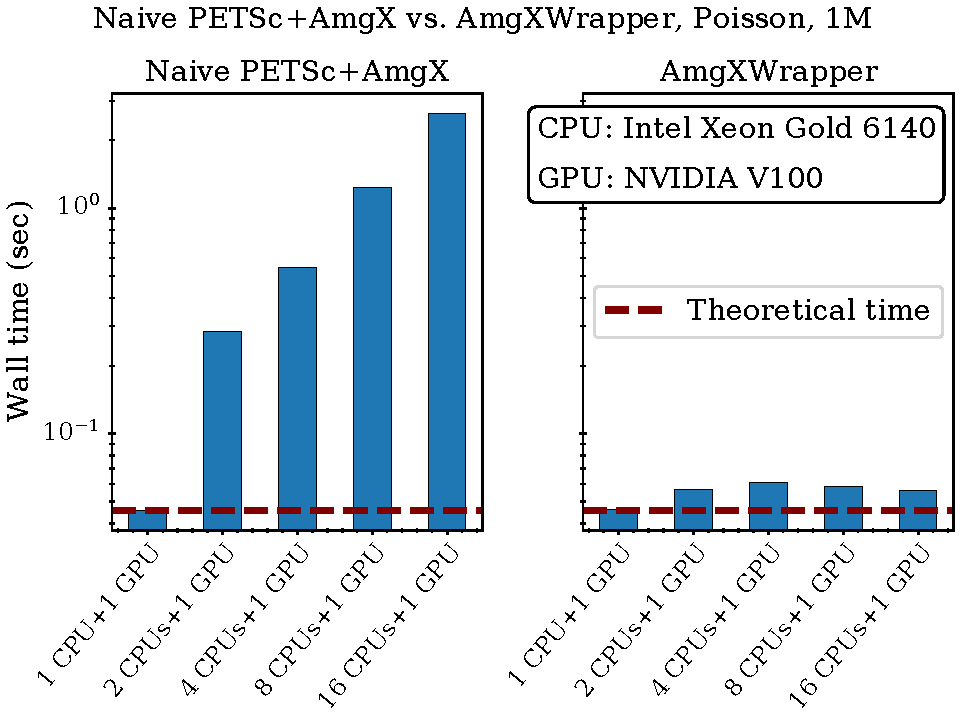
\includegraphics[width=\linewidth]{amgxwrapper-consolidation-tests-poisson-1M}%
    \caption{AmgXWrapper benchmark: 3D Poisson problem w/ 1M unknowns and using 1 V100 GPU.}\label{fig:amgxwrapper-cons-1M}%
\end{figure}
\begin{figure}[hbt!]%
    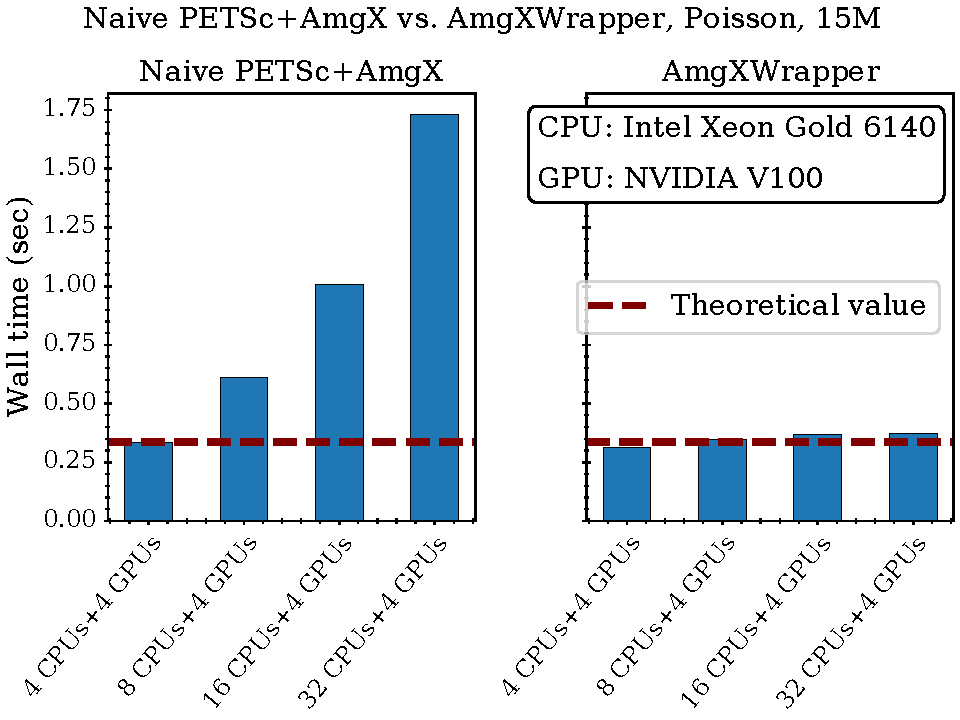
\includegraphics[width=\linewidth]{amgxwrapper-consolidation-tests-poisson-15M}%
    \caption{AmgXWrapper benchmark: 3D Poisson problem w/ 15M unknowns and using 4 V100 GPUs.}\label{fig:amgxwrapper-cons-15M}%
\end{figure}

The left figures of both figures~\ref{fig:amgxwrapper-cons-1M} and~\ref{fig:amgxwrapper-cons-15M} show that using AmgX naively, the wall times increase when the numbers of CPU cores increase. 
The figures on the two subplots' right show that with AmgXWrapper's consolidation mechanism, the wall times remain relatively constant regardless of the numbers of CPU cores.
Please refer to~\cite{chuang_amgxwrapper:_2017} for the explanation of AmgXWrapper's consolidation mechanism.

Figure~\ref{fig:amgxwrapper-speedups} shows the results of speedup/performance benchmarks.
Figure~\ref{fig:amgxwrapper-speedups-15M} shows the speedups of solving a small 3D Poisson problem that fits into one compute node, and figure~\ref{fig:amgxwrapper-speedups-33M} shows that of solving a bigger 3D problem with multiple compute nodes.
The compute nodes have 36 cores of Xeon Gold 6140 CPU cores per node and 4 V100 GPUs per node.
The linear solver used for the CPU results is the BoomerAMG from Hypre~\cite{henson_boomeramg_2002}, which implements the same algorithms used by AmgX but on CPU\@.
Assuming a perfect intra-node scaling of Hypre, one V100 GPU has a performance equivalent to 65 pure CPU cores for the small Poisson problem (figure~\ref{fig:amgxwrapper-speedups-15M}).
However, intra-node scaling is far from perfect, as shown in figure~\ref{fig:amgxwrapper-speedups-15M}.
Therefore, 1 V100 is much more potent than a fat node with 65 CPU cores.
As for the larger problem (figure~\ref{fig:amgxwrapper-speedups-33M}), one node with four GPUs is roughly equivalent to nine pure-CPU nodes.
This estimation assumes the pure-CPU cluster uses low-latency network hardware, such as InfiniBand.
These results imply that using AmgX and GPU computing saves both computational and monetary costs because one standalone workstation of 4 GPUs is cheaper than a 9-node cluster with InfiniBand.
The management cost of one workstation with 4 GPUs is also cheaper than that of a 9-node cluster.

\begin{figure}[hbt!]
    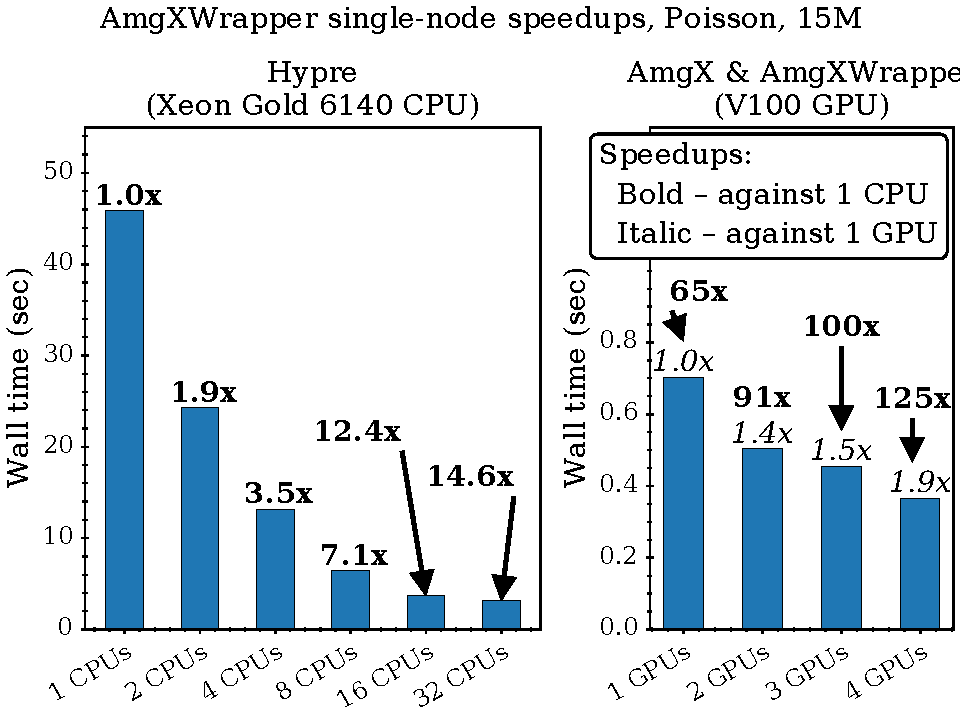
\includegraphics[width=\linewidth]{amgxwrapper-proc-speedups-poisson-15M}
    \caption{Speedups of AmgXWrapper vs.\@ Hypre w/ 15M unknowns.}\label{fig:amgxwrapper-speedups-15M}
\end{figure}

\begin{figure}[hbt!]
    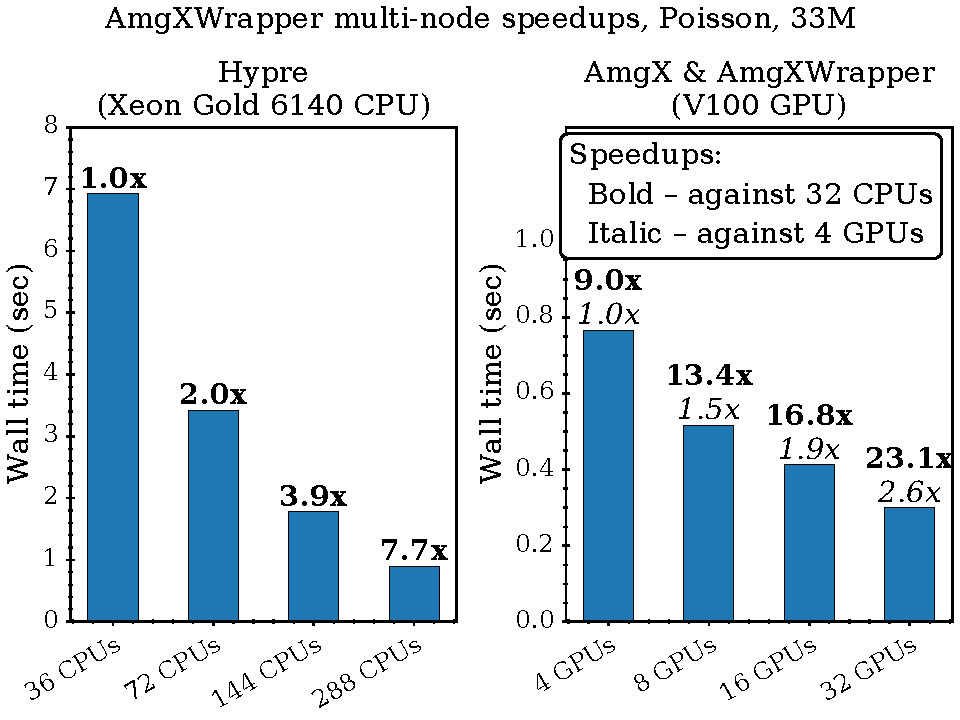
\includegraphics[width=\linewidth]{amgxwrapper-node-speedups-poisson-33M}
    \caption{Speedups of AmgXWrapper vs.\@ Hypre w/ 33M unknowns.}\label{fig:amgxwrapper-speedups-33M}
\end{figure}

% vim:ft=tex


    \section{Verification and Validation}

    \section{Performance Benchmarks}
    %! TEX root = main.tex

PetIBM implements schemes derived from~\cite{Perot1993}, including~\cite{Taira2007} and~\cite{Li2016}.
We presented the numerical schemes and implementation details of PetIBM in~\cite{chuang_petibm:_2018}.
Interested readers can also find verification and validation of PetIBM at reference~\cite{mesnard_petibm_nodate}.
Here we emphasize the performance gain of PetIBM after applying AmgXWrapper.

Figure~\ref{fig:petibm-speedups} shows the performance speedups comparing pure-CPU and CPU-GPU-mixed simulations.
In pure-CPU simulations, PetIBM solves velocity systems with the GAMG preconditioners and pressure systems with BoomerAMG preconditioners.
On the other hand, for CPU-GPU mixed simulations, the preconditioners for velocity and pressure are block-Jacobi and classical multigrid from AmgX, respectively.
The underlying linear system solvers are the biconjugate gradient stabilized solver from either PETSc or AmgX.
All other calculations, including solving the force systems, are done on CPUs.
The two subplots, figure~\ref{fig:petibm-speedups-small} and~\ref{fig:petibm-speedups-large}, represent the results using two different clusters.
Results from both clusters agree with each other.
We can see that a 4-GPU node or 2 2-GPU nodes are equivalent roughly to 5 pure-CPU nodes.
This again proves that adopting GPU computing in PetIBM can reduce both the time and monetary cost of CFD simulations.

% vim:ft=tex


\chapter{Physics-Informed Neural Networks}

    \section{Fundamental of Physics-Informed Neural Networks}

        \subsection{Deep Neural Networks Modeling}
        %! TEX root = main.tex
Consider the incompressible Navier-Stokes equations in a spatial domain of $\vec{x}\in\Omega$ and a time range of $t\in[0$, $T]$:
\begin{subequations}\label{eq:orig-ns}
    \begin{empheq}[left=\left\{\,, right=\right.]{align}
        &\pdiff{\vec{u}}{t} + \left(\vec{u} \cdot \nabla\right) \vec{u}
            =
            -\frac{1}{\rho}\nabla p + \frac{1}{Re} \nabla^2 \vec{u}
            \label{eq:orig-ns-momentum} \\
        &\nabla \cdot \vec{u} = 0 \label{eq:orig-ns-cont}
    \end{empheq}
\end{subequations}
A solution to the Navier-Stokes equations is subject to IC and BCs:
\begin{equation}\label{eq:orig-ns-ic}
    \left\{
        \begin{array}{l}
            \vec{u}(\vec{x}, t=0) = \vec{u}_0(\vec{x}) \\
            p(\vec{x}, t=0) = p_0(\vec{x}) \\
        \end{array}
    \right.
    \text{,\ \ for }
    \vec{x} \in \Omega
\end{equation}
and
\begin{equation}\label{eq:orig-ns-bc}
    \left\{
        \begin{aligned}
            &\vec{u}(\vec{x}, t) = \vec{u}_{bc}(\vec{x}, t) \\
            &p(\vec{x}, t) = p_{bc}(\vec{x}, t)
        \end{aligned}
        \text{,\ \ for }
        \vec{x} \in \Gamma_{bc}
        \text{ and }
        t \in [0, T]
    \right.
\end{equation}
We only list the Dirichlet BCs to save space and for simplicity, as the treatment of Neumann BCs does not differ from treating PDEs in PINNs.

In the method of PINNs, the first step is to approximate the solutions of \eqref{eq:orig-ns} with a neural network model.
Let the network model name be $G$, of which the inputs are spatial coordinates $\vec{x}\equiv\begin{bsmallmatrix}x & y & z\end{bsmallmatrix}^\mathsf{T}$, time $t$, and a set of free parameters $\Theta$ that we need to determine later:
\begin{equation}\label{eq:G-network}
    \begin{bmatrix}
        \vec{u}(\vec{x}, t) \\ p(\vec{x}, t)
    \end{bmatrix}
    \approx
    G(\vec{x}, t; \Theta)
    =
    \begin{bmatrix}
        G^{\vec{u}} \\
        G^p
    \end{bmatrix}
    =
    \begin{bmatrix}
        G^u \\
        G^v \\
        G^w \\
        G^p
    \end{bmatrix}
\end{equation}
where $\vec{u}\equiv\begin{bsmallmatrix}u & v & w\end{bsmallmatrix}^\mathsf{T}$ is the velocity vector, and $p$ is the pressure.
In \eqref{eq:G-network}, we use a single network to predict both pressure and velocity fields.
Though it is possible to use separate networks for different fields, we keep \eqref{eq:G-network} this way for simplicity.
Also, later in this work, we will use $G^{\vec{u}}$, $G^u$, $G^v$, $G^w$, and $G^p$ to denote the predicted velocity vector, components, and pressure from $G$.
In this section, we will focus on the solution workflow \cite{dissanayake_neural-network-based_1994,lagaris_artificial_1998,cai_physics-informed_2021} and leave the mathematical expression of neural network models to section \ref{sec:mlp}.

The next step is to approximate the derivatives required for the differential equations.
For example, the continuity equation $\nabla \cdot \vec{u} = \pdiff{u}{x} + \pdiff{v}{y} + \pdiff{w}{z}$ requires the approximations for the 1st-order derivatives of velocity.
A possible approach is to rely on numerical differentiation.
For example, using finite difference, $\pdiff{u}{x}$ can be
\begin{equation*}
    \pdiff{u}{x} \approx \frac{G^u(x+\Delta x, \cdots)-G^u(x-\Delta x, \cdots)}{2\Delta x} 
\end{equation*}
Model $G$ is continuous and not defined on discretized space, so $x$ can be arbitrary coordinates in the domain.
And $\Delta x$ is a user-provided scalar as there is no grid.
However, we will not proceed with numerical differentiation. 
Being a continuous model and having a well-defined mathematical expression, $G$ gives us two more reasonable options.

The first option is to obtain analytical derivatives through symbolic differentiation or manual derivation.
For example, a very simple MLP network for a steady 2D flow may look like
\begin{equation}\label{eq:explicit-toy-mlp}
    \begin{aligned}
    &\begin{bmatrix}
        u &
        v &
        p
    \end{bmatrix}^\mathsf{T}
    \approx
    \begin{bmatrix}
        G^u &
        G^v &
        G^p
    \end{bmatrix}^\mathsf{T}
    =
    G(x, y; \Theta) \\
    = 
    &\begin{bmatrix}
    c_{11} \cos{\left(a_{11}x + a_{12}y + b_1\right)} + 
      c_{12} \cos{\left(a_{21}x + a_{22}y + b_2\right)} \\
    c_{21} \cos{\left(a_{11}x + a_{12}y + b_1\right)} + 
      c_{22} \cos{\left(a_{21}x + a_{22}y + b_2\right)} \\
    c_{31} \cos{\left(a_{11}x + a_{12}y + b_1\right)} + 
      c_{32} \cos{\left(a_{21}x + a_{22}y + b_2\right)} \\
    \end{bmatrix}
    \end{aligned}
\end{equation}
where $a_{ij}$, $b_i$, and $c_{ki}$ for $i$, $j=1$, $2$ and $k=1$, $2$, $3$ are free parameters in the model and belong to $\Theta$.
This MLP network is said to have one hidden layer with 2 neurons per layer and uses cosine for the activation function.
(Note that it is uncommon to use cosine for activation in real applications.)
We will formally introduce the definitions of these terms and the MLP's matrix form in section \ref{sec:mlp}.
Given the expression of \eqref{eq:explicit-toy-mlp}, we are able to obtain the derivatives.
Such as
\begin{equation}
    \begin{aligned}
    \pdiff{u}{x}
    \approx
    \pdiff{G^u}{x}
    =
    a_{11}c_{11}\cos\left(a_{11}x + a_{12}y + b_1\right) + a_{21}c_{12}\cos\left(a_{21}x + a_{22}y + b_2\right)
    \end{aligned}
\end{equation}
And the same concept applies to all higher-order derivatives.

Analytical derivatives were used in earlier literature when the networks might be just slightly more complicated than the one shown in \eqref{eq:explicit-toy-mlp}.
When the neural network models become more and more complicated, analytical derivatives become much less feasible, if not impossible.
Even modern hardware and symbolic differentiation software may not be able to obtain the analytical derivatives when $G$ has tens of thousands of free parameters and when the activation is not as simple as a cosine function.

Modern deep learning instead relies on the second option: automatic differentiation \cite{griewank_automatic_1988}.
Automatic differentiation is based on the chain rule and gives exact derivatives (exact with respect to actual computer intrinsic operations).
Section \ref{sec:ad} will talk about the fundamental concept of automatic differentiation.
At this point, we can just treat the automatic differentiation as a black box function that returns exact derivatives.
It requires fewer computing resources than symbolic differentiation and provides more accurate derivatives than numerical differentiation.

Moving on to the next step, once we obtain the desired derivatives, we substitute these derivatives into the governing PDEs, IC, and BCs.
For example, by substituting $G$ and corresponding derivatives to \eqref{eq:orig-ns}, \eqref{eq:orig-ns-ic}, and \eqref{eq:orig-ns-bc}, we get several residual functions
\begin{equation}\label{eq:residuals}
    \begin{array}{ll}
        \left\{
            \begin{array}{l}
            \hat{\vec{r}}_{m}(\vec{x}, t; \Theta) \equiv \frac{\partial G^{\vec{u}}}{\partial t}+(G^{\vec{u}} \cdot \nabla) G^{\vec{u}}+\frac{1}{\rho} \nabla G^p -\nu \nabla^{2} G^{\vec{u}} \\
            \hat{r_{c}}(\vec{x}, t; \Theta) \equiv \nabla \cdot G^{\vec{u}} 
            \end{array}
        \right. &
        \forall
        \left\{
            \begin{array}{l}
                \vec{x} \in \Omega \\ t \in [0, T]
            \end{array}
        \right. \\
        \left\{
            \begin{array}{l}
            \hat{\vec{r}}_{ic,\vec{u}}(\vec{x}; \Theta) \equiv G^{\vec{u}}(\vec{x}, t=0)-\vec{u}_0(\vec{x}) \\
            \hat{r}_{ic,p}(\vec{x}; \Theta) \equiv G^{p}(\vec{x}, t=0)-p_0(\vec{x})
            \end{array}
        \right. &
        \forall
        \vec{x} \in \Omega \\
        \left\{
            \begin{array}{l}
            \hat{\vec{r}}_{bc,\vec{u}}(\vec{x}, t; \Theta) \equiv G^{\vec{u}}-\vec{u}_{bc} \\
            \hat{r}_{bc,p}(\vec{x}, t; \Theta) \equiv G^{p}-p_{bc}
            \end{array}
        \right. &
        \forall
        \left\{
            \begin{array}{l}
                \vec{x} \in \Gamma_{bc} \\ t \in [0, T]
            \end{array}
        \right.
    \end{array}
\end{equation}
To make the expression cleaner, we omitted $\vec{x}$, $t$, and $\Theta$ in $G$.
Residual vectors $\hat{\vec{r}}_i$ and residual scalar $\hat{r}_i$, where $i$ denotes different residual sources, are functions of $\vec{x}$, $t$, and $\Theta$.
They are zero anywhere in the domain of interest only when the approximation solution $G$ perfectly fits in \eqref{eq:orig-ns}, \eqref{eq:orig-ns-ic}, and \eqref{eq:orig-ns-bc}.

The final step is to find a set of parameters $\vec{\theta}=\begin{bsmallmatrix}\theta_1 & \theta_2 & \cdots\end{bsmallmatrix}^\mathsf{T}$ that makes all residuals zero, i.e., when $\Theta=\vec{\theta}$, $G$ perfectly fits into \eqref{eq:orig-ns}, \eqref{eq:orig-ns-ic}, and \eqref{eq:orig-ns-bc}.
$\vec{\theta}$ then represents the common zero roots of all the residual functions in \eqref{eq:residuals} for all $\vec{x} \in \Omega$, $\vec{x} \in \Gamma_{bc}$, and $t\in[0$, $T]$.

Assume there are a total of $N_\Theta$ free parameters.
If residual functions in (\ref{eq:residuals}) are not complicated, and if $N_\Theta$ is small enough, we may numerically find the zero roots by solving a system of $N_\Theta$ nonlinear equations.
Such a system of nonlinear equations may be generated by enforcing the zero-residual conditions only on a set of $N_\Theta$ spatial-temporal points, i.e., $N_\Theta$ pairs of $\vec{x}$ and $t$.
However, this approach rarely results in an easy-to-solve system, given that $G$ is usually complicated and $N_\Theta$ is large.
Even for the toy model like \eqref{eq:explicit-toy-mlp}, the first-order derivatives are non-trivial.
If we further consider higher-order derivatives and the native nonlinearity in the PDEs, even this toy model results in a complicated nonlinear system. 
We do not even know if zero roots exist for this nonlinear system.

We instead relax the condition in PINNs.
We do not seek the zero roots of \eqref{eq:residuals} but just hope the desired set of parameters, $\theta$, makes the residuals sufficiently close to zero.
Also, note that the residual functions in \eqref{eq:residuals} are continuous in the domain and time range of our interest.
To make the optimization easier, we also limit ourselves to finding the minimal residuals at some spatial-temporal coordinates only, rather than asking for minimal residuals everywhere in the continuous space-time domain. 
In other words, the resulting optimization problem tries to find $\vec{\theta}$ that gives the minimal residuals on some spatial-temporal points.

Assume we have picked $N_{PDE}$ spatial-temporal points from $\vec{x}\in\Omega$ and $t\in[0$, $T]$, $N_{IC}$ points in $\Omega$ but with a fixed time $t=0$, and $N_{BC}$ points from $\vec{x} \in \Gamma_{bc}$ and $t\in[0$, $T]$.
We define the residuals at these points as \\
\begin{equation}\label{eq:residual-norms}
    \begin{aligned}
        & r_{m}(\Theta) \equiv \sum\limits_{i=1}^{N_{PDE}} \lVert\frac{\partial G_i^{\vec{u}}}{\partial t}+(G_i^{\vec{u}} \cdot \nabla) G_i^{\vec{u}}+\frac{1}{\rho} \nabla G_i^p -\nu \nabla^{2} G_i^{\vec{u}} \rVert^2 \\
        & r_{c}(\Theta) \equiv \sum\limits_{i=1}^{N_{PDE}} ( \nabla \cdot G_i^{\vec{u}} )^2 \\
        & r_{ic,\vec{u}}(\Theta) \equiv \sum\limits_{i=1}^{N_{IC}} \lVert G^{\vec{u}}(\vec{x}_i, t=0)-\vec{u}_0(\vec{x}_i) \rVert^2 \\
        & r_{ic,p}(\Theta) \equiv \sum\limits_{i=1}^{N_{IC}} ( G^{p}(\vec{x}_i, t=0)-p_0(\vec{x}_i) )^2 \\
        & r_{bc,\vec{u}}(\Theta) \equiv \sum\limits_{i=1}^{N_{BC}} \lVert G_i^{\vec{u}}-\vec{u}_{bc} \rVert^2 \\
        & r_{bc,p}(\Theta) \equiv \sum\limits_{i=1}^{N_{BC}} ( G_i^{p}-p_{bc} )^2
   \end{aligned}
\end{equation}
where $\begin{bsmallmatrix}G_i^{\vec{u}} & G_i^p\end{bsmallmatrix}^\mathsf{T} = G(\vec{x}_i, t_i; \Theta)$, and $\lVert\cdot\rVert$ denotes $l_2$ norms.

One approach to interpret the optimization problem is
\begin{equation}\label{eq:hard-constraint-loss}
    \begin{aligned}
    &\vec{\theta} = \operatorname*{arg\,min}\limits_{\Theta} \left[r_m(\Theta) + r_c(\Theta)\right] \\
    \text{ subject to } &r_{ic,\vec{u}}=r_{ic,p}=r_{bc,\vec{u}}=r_{bc,p}=0
    \end{aligned}
\end{equation}
This is a constrained optimization problem.
Only residuals from PDEs are relaxed, and residuals from BCs and IC must be exactly zero.
Though exactly satisfied BCs and IC sound attractive, optimization with hard constraints is much more difficult than unconstrained optimization.
And optimization methods may not be general enough for arbitrary types of BCs and arbitrary computational domains.
This approach was used in, for example, references \cite{lagaris_artificial_1998,McFall2009,mcfall_solving_2010,berg_unified_2018} for limited types of PDEs and applications.

Alternatively, most recent reports of PINNs used soft constraints, that is
\begin{equation}\label{eq:total-residual}
    \vec{\theta} = \operatorname*{arg\,min}\limits_{\Theta} \left[
        r_m(\Theta) + r_c(\Theta) + r_{ic,\vec{u}}(\Theta) + r_{ic,p}(\Theta) + r_{bc,\vec{u}}(\Theta) + r_{bc,p}(\Theta)
    \right]
\end{equation}
Though the optimized $\vec{\theta}$ does not guarantee that IC and BCs are satisfied, \eqref{eq:total-residual} is easier to solve and to be generalized to different PDEs, BCs, or applications.
In the terminology of optimization, \eqref{eq:total-residual} is called the loss function or objective.
Residuals from different sources are called loss terms.

In practice, a more general form of \eqref{eq:total-residual} is
\begin{equation}\label{eq:total-residual-weighted}
    \begin{aligned}
        \vec{\theta}
        &=
        \operatorname*{arg\,min}\limits_{\Theta} r(\Theta)  \\
        &=
        \operatorname*{arg\,min}\limits_{\Theta} \sum \alpha_i r_i(\Theta)
    \end{aligned}
\end{equation}
where $i$ denotes different loss terms in \eqref{eq:residual-norms}.
Each loss term is weighted before being aggregated to the final loss.
To our best knowledge, there is not yet a standard or guideline for how to properly configure $\alpha_i$.
It is common to see $\alpha_i=1$ in the literature.

If there exist zero roots that make all residuals in \eqref{eq:residual-norms} zero, then a perfect optimization method will find them from either \eqref{eq:hard-constraint-loss}, \eqref{eq:total-residual}, or \eqref{eq:total-residual-weighted}.
This hope is surely unrealistic.
First, zero roots' existence is not guaranteed.
Second, the hypersurface of the aggregated loss, $r(\Theta)$, in the vector space of $\Theta$ is usually neither convex nor concave, making it difficult to find the global minimum.
Even a simple 1D linear Burger's equation with an MLP of around \num{7850} free model parameters shows a complicated hypersurface of $r(\Theta)$ \cite{krishnapriyan_characterizing_2021}.
While finding zero roots or the global minimum on the hypersurface of $r(\Theta)$ is difficult, practitioners of PINNs just assume the local minimums of $r(\Theta)$ are good and small enough.

This poses a fundamental difference between conventional CFD schemes and PINNs: the former seeks exact zero roots to make residuals zero, while the latter just {\it hopes} to make residuals as small as possible.
It is thus reasonable to doubt PINNs' accuracy compared to conventional schemes.

Nevertheless, finding optimized $\vec{\theta}$ concludes the workflow of data-free PINNs for solving PDEs.
Figure \ref{fig:pinn-workflow} shows a graphical illustration of the workflow.
\begin{figure}[hbt!]
    \includegraphics[width=\linewidth]{figs/pinn.tikz} 
    \caption{A graphical demonstration of workflow in PINNs}
    \label{fig:pinn-workflow}
\end{figure}

The optimization process is done with the Adam optimizer \cite{kingma_adam_2017} in this work, together with a batched approach described in the next section.
% vim:ft=tex


        \subsection{Periodic Boundaries}\label{section:periodic-boundary}

        \subsection{Remark on difference and similarities with conventional numerical methods}
        %! TEX root = main.tex

Compared to solving $N_\Theta$ nonlinear equations directly, an optimization problem of \eqref{eq:total-residual} or \eqref{eq:total-residual-weighted} allows us to use any number of spatial-temporal points.
That is, there is no limitation on the magnitude of $N_{PDE}$, $N_{BC}$, and $N_{IC}$.
This eases the need for computational resources.
In data-free PINNs, these spatial-temporal points are called training points or training data.
They are spatial-temporal coordinates where we evaluate the residuals of PDEs, IC, and BCs.
While training points may be generated manually and intentionally positioned at desired locations (just like meshing in conventional CFD simulations), it is more common to generate them by selecting coordinates randomly using a uniform density function. 

The ability to use arbitrary numbers of training points helps the generalizability of a trained PINNs model.
When more training points are involved in \eqref{eq:residual-norms} and hence \eqref{eq:total-residual-weighted}, the minimal residuals are achieved at more locations in the domain. 
Ultimately, with unlimited training points evenly distributed in the domain, optimizing the discretized residuals in \eqref{eq:residual-norms} becomes optimizing continuous residual functions in \eqref{eq:residuals}. 
And the resulting optimal parameters, $\vec{\theta}$, will make $G$ a more accurate approximation solution to the whole domain of $\Omega$ and $t\in[0$, $T]$.

More points also mean a higher computational cost.
Batched training is thus utilized to reduce the cost.
For example, if using an iterative optimization method (such as the gradient-descent or Adam optimizer), we can always generate a new batch of training points for a new iteration to evaluate the discretized residuals.
After a significant number of iterations, the total number of training points involved in optimization will also be significant.
Once the model is trained, theoretically, it is capable of giving accurate predictions at any location and time.

In practice, however, it is not a cheap task if thousands or even more random points have to be generated on the fly at each iteration.
We instead generated a fixed amount of training points before the optimization and only used a batch of them in each iteration.
For example, to use $N_{PDE}$ points to evaluate the PDE residuals at each iteration, we may generate $N_{PDE}\times 1000$ points in advance and divide them into $1000$ batches.
If we run an optimizer for 1 million iterations, each batch is repeated every 1000 iterations.

Theoretically, each batch should have similar statistical properties and give a similar gradient vector under fixed model parameters.
That is
\begin{equation}
\left.\nabla_\theta r(\Theta) \right|_{\vec{x}, t \in \mathcal{X}_1} \sim
\left.\nabla_\theta r(\Theta) \right|_{\vec{x}, t \in \mathcal{X}_2} \sim
\cdots
\end{equation}
where $\mathcal{X}_i$ for $i=1$, $2$, $\cdots$ represents the $i$-th batch of the training points.
These gradients are used to update $\vec{\theta}$ in iterative optimization methods.
In other words, the hypersurface of $r(\Theta)$ is expected not to change significantly from iteration to iteration when using different batches of points to evaluate it.
However, whether this statement is true may depend on the number of points in each batch: the number of points should be large enough to have similar statistical properties across different batches.

In PINNs, as the training points are randomly sampled from the computational space-time domain, the number of points in a batch should be large enough to cover all over the domain.
Otherwise, for example, if one batch mostly covers the inflow region of a cylinder flow while the next batch covers mostly the wake region behind the cylinder, then the hypersurface of the PDE residuals will change significantly.
This change of the hypersurface from iteration to iteration may slow down the convergence.
In the later benchmarks, we would like to examine the effect of batch sizes, i.e., the number of points in each batch. 

% vim:ft=tex


        \subsection{Automatic Differentiation}
        %! TEX root = main.tex
In equation \eqref{eq:total-residual-weighted}, each individual loss term is weighted.
However, how to properly assign the weights is still and open question.
In references \cite{jin_nsfnets_2020,wang_understanding_2021}, the authors proposed an annealing approach to change these weights in an adaptive fashion during the optimization process.
However, these adaptive approaches have not been further tested by more works.
In this work, part of the benchmarks will cover the performance of the adaptive weight strategy proposed in \cite{jin_nsfnets_2020}.

Jin et al. \cite{jin_nsfnets_2020} proposed the following annealing loss aggregation algorithm for iterative optimization methods:
\begin{equation}
    r^k(\Theta) = r_{PDE}^k(\Theta) + 
        \left(\left(1-\lambda\right)\alpha^k + \lambda\alpha^{k+1}\right)r_{BC}^k(\Theta) + 
        \left(\left(1-\lambda\right)\beta^k + \lambda\beta^{k+1}\right)r_{IC}^k(\Theta)
\end{equation}
where $k$ denotes the $k$-th iteration in an iterative optimization method.
The subscript $PDE$, $BC$, and $IC$ denote the loss contributions from the residuals of PDEs, BCs, and IC.
$\lambda$ is a user-provided parameter to control the moving average of the current and the previous weights.
The concept of this adaptive approach is to make the gradients of each loss term comparable.
When using the gradient-descent method and its derived methods, the magnitude of each loss term is reduced with a similar rate.
And
\begin{equation}
    \alpha^{k+1} = \frac{\overline{\lvert\nabla_\Theta r_{PDE}^k(\Theta)\rvert}}{\overline{\lvert\nabla_\Theta r_{BC}^k(\Theta)\rvert}}
    \text{\ \ \ \ and\ \ \ \ }
    \beta^{k+1} = \frac{\overline{\lvert\nabla_\Theta r_{PDE}^k(\Theta)\rvert}}{\overline{\lvert\nabla_\Theta r_{IC}^k(\Theta)\rvert}}
\end{equation}
$\lvert\cdot\rvert$ denotes the element-wise absolute values of a vector.
$\overline{\lvert\cdot\rvert}$ is the mean values of these absolute values.

The following expression better represents the actual implementation in our code:
\begin{equation}
    \begin{aligned}
        &\zeta^k =
            \overline{\lvert\nabla_\Theta r_{m,u}^k(\Theta)\rvert} +
            \overline{\lvert\nabla_\Theta r_{m,v}^k(\Theta)\rvert} +
            \overline{\lvert\nabla_\Theta r_{m,w}^k(\Theta)\rvert} +
            \overline{\lvert\nabla_\Theta r_{c}^k(\Theta)\rvert} \\
        &\alpha^{k+1} = 
            \frac{\zeta^k}{\overline{\lvert\nabla_\Theta r_i^k(\Theta)\rvert}} \\
        &r^k(\Theta) = r_m^k(\Theta) + r_c^k(\Theta) + 
            \sum\limits_{i} \left(\left(1-\lambda\right)\alpha_i^k + \lambda\alpha_i^{k+1}\right) r_i^k(\Theta)
    \end{aligned}
\end{equation}
where $r_{m,u}^k$, $r_{m,v}^k$, and $r_{m,w}^k$ are the $u$-, $v$-, and $w$-component in the residual vector of the momentum equations at $k$-th iteration.
And subscript $i$ denotes different loss terms, excluding $r_m(\Theta)^k$ and $r_c(\Theta)^k$.
In this work, $\lambda$ is fixed at $0.1$ for all cases using annealing loss aggregation.
% vim:ft=tex

        \subsection{Adaptive Loss Reduction}\label{section:loss-annealing}
        %! TEX root = main.tex

% vim:ft=tex


    \section{Adam Optimizer, Batched Training, and Cyclical Learning Rates}\label{section:adam}

    \section{Nonlinear Conjugate-Gradient Optimizer and Line Search}

    \section{Stochastic Weight Averaging and Training Strategy}

\chapter{Computational Experiments Configurations and Results}

    \section{2D Taylor-Green Vortex and Configurations}
    %! TEX root = main.tex

\subsection{Problem description}

The Taylor-Green vortex (TGV) represents a family of flows with a specific form of analytical initial flow conditions in both 2D and 3D.
Specifically, 2D TGV problems with periodic boundary conditions have closed-form analytical solutions, and hence they are standard benchmark cases for verifying CFD solvers. 
In the follow sections, we used the following 2D TGV problem to investigate several different aspects of the PINN method:
\begin{equation}\label{eq:tgv}
    \left\{
        \begin{aligned}
            u(x, y, t) &= V_0\cos(\frac{x}{L})\sin(\frac{y}{L})\exp(-2\frac{\nu}{L^2}t) \\
            v(x, y, t) &= - V_0 \sin(\frac{x}{L})\cos(\frac{y}{L})\exp(-2\frac{\nu}{L^2}t) \\
            p(x, y, t) &= -\frac{\rho}{4}V_0^2\left(cos(\frac{2x}{L}) + cos(\frac{2y}{L})\right)\exp(-4\frac{\nu}{L^2}t)
        \end{aligned}
    \right.
\end{equation}

\noindent $V_0$ represents the peak (and also the lowest) velocity at $t=0$;
$L$ is a scaling factor in the spatial domain;
$\nu$ and $\rho$ are kinematic viscosity and density, respectively.
$u$ and $v$ denote the velocity components in $x$ and $y$ directions.
$p$ is the pressure.
The periodic boundary conditions are applied to $x=-L\pi$, $x=L\pi$, $y=-L\pi$, and $y=L\pi$.

We used the following parameters for all our computational experiments: $V_0=L=\rho=1.0$ and $\nu=0.01$.
These parameters correspond to a Reynolds number of $Re=100$.
Figure \ref{fig:tgv-analytical-demo} shows the snapshots of the analytical solutions at $t=40$ and $t=80$..
\begin{figure}[H]
    \centering
    \includegraphics{tgv-2d-re100/tgv-re100-analytical-demo}%
    \caption{Contours of the analytical solutions of 2D TGV ($Re=100$) at $t=40$ and $t=80$ for demonstration.}\label{fig:tgv-analytical-demo}
\end{figure}

\noindent As shown in the figure and in the analytical solutions, the flow patterns do not change spatially, and only the amplitudes decay exponentially in time.

This TGV problem serves as a good benchmark case because it reduces the number of required residual constraints in PINNs.
Periodic boundary conditions eliminates the constraints coming from boundary conditions.
Rather, modified input coordinates are used as described in section \ref{section:periodic-boundary}.
The optimizer hence can focus only on the residuals of initial conditions and the Navier-Stokes equations.
The training process should be easier, compared to other more realistic flow problems.

\subsection{Solver configuration}

The neural network used in the PINN solver is a weight-normalization fully-connected neural network.
The benchmarks cases cover the numbers of hidden layers ranging from 1 to 3 layers, i.e., $N_l=1$, $2$, and $3$.
Each number of hidden layers have neurons per layer ranging from 16 to 256 (that is , $N_n=2^k$ for $k=4, 5, \cdots, 8$.
The activation functions are SiLU \cite{hendrycks_gaussian_2016}.
See equation \ref{eq:silu}.

The training processes are the same for all cases: 100,000 iterations of Adam optimization and 200 iterations of CG optimization.
Adam training is as described in section \ref{section:adam}.
The benchmarks in this section all use exponentially decaying learning rates: at $i$-th iteration, the learning rate is
\begin{equation}
    lr(i) = 0.95^\frac{i}{5000}
\end{equation}
The Adam optimizer itself has $\beta_1=0.9$, $\beta_2=0.999$, and $\epsilon=10^{-8}$.
We used annealing loss aggregation algorithm to sum up different residuals sources.
See section \ref{section:loss-annealing}.

Aside from the changes in network architectures, we also investigated the effect of the number of training points used per iteration (i.e., the batch size, $N_{bs}$).
7 different batch sizes were used for each architecture, that is, $N_{bs}=2^m$ for $m=10, 11, \cdots, 16$.
The solver pre-generated $1000 \times N_{bs}$ spatial-temporal points and only used $N_{bs}$ in each iteration.
In other words, running through the whole dataset takes 1,000 iterations.
These training points were randomly sampled from the spatial domain $[-\pi, \pi]\times[-\pi, \pi]$ and temporal domain $(0, 100]$.

In addition to the PDE residual evaluation points, the solver also pre-generated $1000 \times N_{bs}$ random points to evaluate the residuals of the initial conditions.
Note that for the initial condition, the evaluation points were sampled from the spatial domain only because $t=0$ is a fixed condition.
Because of the periodic boundary conditions, the solver does not require any training points for boundary conditions.

In sum, combining the changes in $N_l$, $N_n$, and $N_{bs}$, we ran a total of 105 cases for this 2D TGV problem.

The hardware used for the PINN solver were NVIDIA's V100 GPUs.
Except for the scaling benchmarks, all other benchmarks ran on only one GPU.

After training, the PINN solver's prediction errors (i.e., accuracy) were evaluated on cell centers of a $512 \times 512$ Cartesian mesh against the analytical solutions.
With these spatially distributed errors, we calculated the $L_2$ error norm for a given $t$.
For example, the $L_2$ error of $u$ is calculated by
\begin{equation}\label{eq:l2norm}
    L_2(t)
    =
    \sqrt{\int\limits_{\Omega} u_{err}(x, y, t)^2 \diff\Omega}
    \approx
    \sqrt{\sum\limits_{i}\sum\limits_{j} \left(u_{PINN}\left(x_i, y_j, t\right)-u_{analytical}\left(x_i, y_j, t\right)\right)^2 \Delta \Omega_{i, j}}
\end{equation}

\noindent where $i$ and $j$ are the indices of a cell center in the Cartesian mesh. $\Delta\Omega_{i,j}$ is the corresponding cell area, which is $4\pi^2/512^2$ in this case.

Some results are compared against those from PetIBM simulations.
All PetIBM simulations were done with 1 K40 GPU and 6 CPU cores (Intel i7-5930K).
We carried out 7 PetIBM simulations with different spatial resolutions: $2^k\times 2^k$ for $k=4, 5, \dots, 10$.
The time step size for each spatial resolution was $\Delta t=0.1/2^{k-4}$.

A special note should be made here: the PINN solver used single-precision floats, while PetIBM used double-precision floats.
This discrepancy does not change the qualitative findings and conclusions we will see in later sections.

\subsection{Training Histories and Results Visualization}

In this section, we present the training histories and basic result visualizations for some of the cases.
The selected cases are all $N_{bs}$ under architectures $(N_l, N_n)=(1, 16)$, $(1, 256)$, $(3, 16)$, and $(3, 256)$.
These are the edge cases in $N_l$-$N_n$ space.
We hope to have a qualitative insight toward the bounds of the accuracy and performance in $N_l$-$N_n$ space.

Figures \ref{fig:nl1-nn16-u-err-contour},  \ref{fig:nl1-nn256-u-err-contour}, \ref{fig:nl3-nn16-u-err-contour}, and \ref{fig:nl3-nn256-u-err-contour} show the error contours of $u$ for the selected cases.
We leave the similar visualizations for other fields and other architectures in Appendix \ref{section:extra-data}.

\begin{figure}[H]
    \centering%
    \floatbox{figure}{%
        \begin{subfloatrow}[2]%
            \ffigbox[\FBwidth]{%
                \includegraphics[width=0.45\textwidth]{tgv-2d-re100/training-hist/fixed-arch-loss-nl1-nn16}%
            }{%
                \caption{$(N_l, N_n)=(1, 16)$}\label{fig:nl1-nn16-loss-hist}%
            }%
            \ffigbox[\FBwidth]{%
                \includegraphics[width=0.45\textwidth]{tgv-2d-re100/training-hist/fixed-arch-loss-nl1-nn256}%
            }{%
                \caption{$(N_l, N_n)=(1, 256)$}\label{fig:nl1-nn256-loss-hist}%
            }%
        \end{subfloatrow}%

        \begin{subfloatrow}[2]%
            \ffigbox[\FBwidth]{%
                \includegraphics[width=0.45\textwidth]{tgv-2d-re100/training-hist/fixed-arch-loss-nl3-nn16}%
            }{%
                \caption{$(N_l, N_n)=(3, 16)$}\label{fig:nl3-nn16-loss-hist}%
            }%
            \ffigbox[\FBwidth]{%
                \includegraphics[width=0.45\textwidth]{tgv-2d-re100/training-hist/fixed-arch-loss-nl3-nn256}%
            }{%
                \caption{$(N_l, N_n)=(3, 256)$}\label{fig:nl3-nn256-loss-hist}%
            }%
        \end{subfloatrow}%
    }{%
        \caption{Training history (aggregated loss) of selected architectures.}\label{fig:loss-hist}%
    }%
\end{figure}

\begin{figure}[H]
    \includegraphics{tgv-2d-re100/contours/nl1-nn16/nl1-nn16-orig-u}
    \caption{Spatial distributions of errors for architecture $(N_l, N_n)=(1, 16)$.}\label{fig:nl1-nn16-u-err-contour}
\end{figure}

\begin{figure}[H]
    \includegraphics{tgv-2d-re100/contours/nl1-nn256/nl1-nn256-orig-u}
    \caption{Spatial distributions of errors for architecture $(N_l, N_n)=(1, 256)$.}\label{fig:nl1-nn256-u-err-contour}
\end{figure}

\begin{figure}[H]
    \includegraphics{tgv-2d-re100/contours/nl3-nn16/nl3-nn16-orig-u}
    \caption{Spatial distributions of errors for architecture $(N_l, N_n)=(3, 16)$.}\label{fig:nl3-nn16-u-err-contour}
\end{figure}

\begin{figure}[H]
    \includegraphics{tgv-2d-re100/contours/nl3-nn256/nl3-nn256-orig-u}
    \caption{Spatial distributions of errors for architecture $(N_l, N_n)=(3, 256)$.}\label{fig:nl3-nn256-u-err-contour}
\end{figure}


\subsection{Optimal Batch Size Investigation}
\subsection{Loss and Accuracy versus Model Complexity}
\subsection{Performance and Scalability}

% vim:ft=tex


    \section{Vanilla Summation versus Annealing Loss Aggregation}

    \section{Exponentially Decayed versus Cyclical Learning Rates}
    The upper and lower bounds for cycling learning rates are $10^{-3}$ and $10^{-6}$, while one cycle takes 4000 iterations.

    \section{Unsteady Flow Problems}

\chapter{Discussion and Future Works}

\appendix
\chapter{Extra Data and Visualizations for 2D Taylor-Green Vortex Benchmarks}\label{section:extra-data}
%! TEX root = main.tex

% the overview table, the label is `table:tgv-overview`
\begin{landscape}
    \singlespacing
    \scriptsize
    \centering
    \input{tables/tgv-data-overview.tex}
\end{landscape}

% training histories, nl=1, nn=16 to 256
\begin{figure}[H]
    \centering
    \vfill
    \includegraphics[width=0.475\linewidth, height=0.3\textheight]{tgv-2d-re100/training-hist/fixed-arch-loss-nl1-nn16}%
    \hfill
    \includegraphics[width=0.475\linewidth, height=0.3\textheight]{tgv-2d-re100/training-hist/fixed-arch-loss-nl1-nn32}%
    \newline
    \includegraphics[width=0.475\linewidth, height=0.3\textheight]{tgv-2d-re100/training-hist/fixed-arch-loss-nl1-nn64}%
    \hfill
    \includegraphics[width=0.475\linewidth, height=0.3\textheight]{tgv-2d-re100/training-hist/fixed-arch-loss-nl1-nn128}%
    \newline
    \includegraphics[width=0.475\linewidth, height=0.3\textheight]{tgv-2d-re100/training-hist/fixed-arch-loss-nl1-nn256}%
    \caption{Training histories of architectures $N_l=1$ and $N_n=16,32,64,128,256$}
\end{figure}

% training histories, nl=2, nn=16 to 256
\begin{figure}[H]
    \centering
    \includegraphics[width=0.475\linewidth, height=0.3\textheight]{tgv-2d-re100/training-hist/fixed-arch-loss-nl2-nn16}%
    \hfill
    \includegraphics[width=0.475\linewidth, height=0.3\textheight]{tgv-2d-re100/training-hist/fixed-arch-loss-nl2-nn32}%
    \newline
    \includegraphics[width=0.475\linewidth, height=0.3\textheight]{tgv-2d-re100/training-hist/fixed-arch-loss-nl2-nn64}%
    \hfill
    \includegraphics[width=0.475\linewidth, height=0.3\textheight]{tgv-2d-re100/training-hist/fixed-arch-loss-nl2-nn128}%
    \newline
    \includegraphics[width=0.475\linewidth, height=0.3\textheight]{tgv-2d-re100/training-hist/fixed-arch-loss-nl2-nn256}%
    \caption{Training histories of architectures $N_l=2$ and $N_n=16,32,64,128,256$}
\end{figure}

% training histories, nl=3, nn=16 to 256
\begin{figure}[H]
    \centering
    \includegraphics[width=0.475\linewidth, height=0.3\textheight]{tgv-2d-re100/training-hist/fixed-arch-loss-nl3-nn16}%
    \hfill
    \includegraphics[width=0.475\linewidth, height=0.3\textheight]{tgv-2d-re100/training-hist/fixed-arch-loss-nl3-nn32}%
    \newline
    \includegraphics[width=0.475\linewidth, height=0.3\textheight]{tgv-2d-re100/training-hist/fixed-arch-loss-nl3-nn64}%
    \hfill
    \includegraphics[width=0.475\linewidth, height=0.3\textheight]{tgv-2d-re100/training-hist/fixed-arch-loss-nl3-nn128}%
    \newline
    \includegraphics[width=0.475\linewidth, height=0.3\textheight]{tgv-2d-re100/training-hist/fixed-arch-loss-nl3-nn256}%
    \caption{Training histories of architectures $N_l=3$ and $N_n=16,32,64,128,256$}
\end{figure}

% continuity residuals v.s. iterations, nl=1, nn=16 to 256
\begin{figure}[H]
    \centering
    \includegraphics[width=0.475\linewidth, height=0.3\textheight]{tgv-2d-re100/training-hist/fixed-arch-cont_res-nl1-nn16}%
    \hfill
    \includegraphics[width=0.475\linewidth, height=0.3\textheight]{tgv-2d-re100/training-hist/fixed-arch-cont_res-nl1-nn32}%
    \newline
    \includegraphics[width=0.475\linewidth, height=0.3\textheight]{tgv-2d-re100/training-hist/fixed-arch-cont_res-nl1-nn64}%
    \hfill
    \includegraphics[width=0.475\linewidth, height=0.3\textheight]{tgv-2d-re100/training-hist/fixed-arch-cont_res-nl1-nn128}%
    \newline
    \includegraphics[width=0.475\linewidth, height=0.3\textheight]{tgv-2d-re100/training-hist/fixed-arch-cont_res-nl1-nn256}%
    \caption{Change of the residuals of the continuity equation during training. Architectures $N_l=1$ and $N_n=16,32,64,128,256$}
\end{figure}

% continuity residuals v.s. iterations, nl=2, nn=16 to 256
\begin{figure}[H]
    \centering
    \includegraphics[width=0.475\linewidth, height=0.3\textheight]{tgv-2d-re100/training-hist/fixed-arch-cont_res-nl2-nn16}%
    \hfill
    \includegraphics[width=0.475\linewidth, height=0.3\textheight]{tgv-2d-re100/training-hist/fixed-arch-cont_res-nl2-nn32}%
    \newline
    \includegraphics[width=0.475\linewidth, height=0.3\textheight]{tgv-2d-re100/training-hist/fixed-arch-cont_res-nl2-nn64}%
    \hfill
    \includegraphics[width=0.475\linewidth, height=0.3\textheight]{tgv-2d-re100/training-hist/fixed-arch-cont_res-nl2-nn128}%
    \newline
    \includegraphics[width=0.475\linewidth, height=0.3\textheight]{tgv-2d-re100/training-hist/fixed-arch-cont_res-nl2-nn256}%
    \caption{Change of the residuals of the continuity equation during training. Architectures $N_l=2$ and $N_n=16,32,64,128,256$}
\end{figure}

% continuity residuals v.s. iterations, nl=3, nn=16 to 256
\begin{figure}[H]
    \centering
        \includegraphics[width=0.475\linewidth, height=0.3\textheight]{tgv-2d-re100/training-hist/fixed-arch-cont_res-nl3-nn16}%
    \hfill
        \includegraphics[width=0.475\linewidth, height=0.3\textheight]{tgv-2d-re100/training-hist/fixed-arch-cont_res-nl3-nn32}%
    \hfill
        \includegraphics[width=0.475\linewidth, height=0.3\textheight]{tgv-2d-re100/training-hist/fixed-arch-cont_res-nl3-nn64}%
    \hfill
        \includegraphics[width=0.475\linewidth, height=0.3\textheight]{tgv-2d-re100/training-hist/fixed-arch-cont_res-nl3-nn128}%
    \newline
        \includegraphics[width=0.475\linewidth, height=0.3\textheight]{tgv-2d-re100/training-hist/fixed-arch-cont_res-nl3-nn256}%
    \caption{Change of the residuals of the continuity equation during training. Architectures $N_l=3$ and $N_n=16,32,64,128,256$}
\end{figure}

% momentum x residuals v.s. iterations, nl=1, nn=16 to 256
\begin{figure}[H]
    \centering
        \includegraphics[width=0.475\linewidth, height=0.3\textheight]{tgv-2d-re100/training-hist/fixed-arch-momem_x_res-nl1-nn16}%
    \hfill
        \includegraphics[width=0.475\linewidth, height=0.3\textheight]{tgv-2d-re100/training-hist/fixed-arch-momem_x_res-nl1-nn32}%
    \newline
        \includegraphics[width=0.475\linewidth, height=0.3\textheight]{tgv-2d-re100/training-hist/fixed-arch-momem_x_res-nl1-nn64}%
    \hfill
        \includegraphics[width=0.475\linewidth, height=0.3\textheight]{tgv-2d-re100/training-hist/fixed-arch-momem_x_res-nl1-nn128}%
    \newline
        \includegraphics[width=0.475\linewidth, height=0.3\textheight]{tgv-2d-re100/training-hist/fixed-arch-momem_x_res-nl1-nn256}%
    \caption{Change of the residuals in $x$ momentum equation during training. Architectures $N_l=1$ and $N_n=16,32,64,128,256$}
\end{figure}

% momentum x residuals v.s. iterations, nl=2, nn=16 to 256
\begin{figure}[H]
    \centering
        \includegraphics[width=0.475\linewidth, height=0.3\textheight]{tgv-2d-re100/training-hist/fixed-arch-momem_x_res-nl2-nn16}%
    \hfill
        \includegraphics[width=0.475\linewidth, height=0.3\textheight]{tgv-2d-re100/training-hist/fixed-arch-momem_x_res-nl2-nn32}%
    \newline
        \includegraphics[width=0.475\linewidth, height=0.3\textheight]{tgv-2d-re100/training-hist/fixed-arch-momem_x_res-nl2-nn64}%
    \hfill
        \includegraphics[width=0.475\linewidth, height=0.3\textheight]{tgv-2d-re100/training-hist/fixed-arch-momem_x_res-nl2-nn128}%
    \newline
        \includegraphics[width=0.475\linewidth, height=0.3\textheight]{tgv-2d-re100/training-hist/fixed-arch-momem_x_res-nl2-nn256}%
    \caption{Change of the residuals in $x$ momentum equation during training. Architectures $N_l=2$ and $N_n=16,32,64,128,256$}
\end{figure}

% momentum x residuals v.s. iterations, nl=3, nn=16 to 256
\begin{figure}[H]
    \centering
        \includegraphics[width=0.475\linewidth, height=0.3\textheight]{tgv-2d-re100/training-hist/fixed-arch-momem_x_res-nl3-nn16}%
    \hfill
        \includegraphics[width=0.475\linewidth, height=0.3\textheight]{tgv-2d-re100/training-hist/fixed-arch-momem_x_res-nl3-nn32}%
    \hfill
        \includegraphics[width=0.475\linewidth, height=0.3\textheight]{tgv-2d-re100/training-hist/fixed-arch-momem_x_res-nl3-nn64}%
    \hfill
        \includegraphics[width=0.475\linewidth, height=0.3\textheight]{tgv-2d-re100/training-hist/fixed-arch-momem_x_res-nl3-nn128}%
    \newline
        \includegraphics[width=0.475\linewidth, height=0.3\textheight]{tgv-2d-re100/training-hist/fixed-arch-momem_x_res-nl3-nn256}%
    \caption{Change of the residuals in $x$ momentum equation during training. Architectures $N_l=3$ and $N_n=16,32,64,128,256$}
\end{figure}

% momentum y residuals v.s. iterations, nl=1, nn=16 to 256
\begin{figure}[H]
    \centering
        \includegraphics[width=0.475\linewidth, height=0.3\textheight]{tgv-2d-re100/training-hist/fixed-arch-momem_y_res-nl1-nn16}%
    \hfill
        \includegraphics[width=0.475\linewidth, height=0.3\textheight]{tgv-2d-re100/training-hist/fixed-arch-momem_y_res-nl1-nn32}%
    \newline
        \includegraphics[width=0.475\linewidth, height=0.3\textheight]{tgv-2d-re100/training-hist/fixed-arch-momem_y_res-nl1-nn64}%
    \hfill
        \includegraphics[width=0.475\linewidth, height=0.3\textheight]{tgv-2d-re100/training-hist/fixed-arch-momem_y_res-nl1-nn128}%
    \newline
        \includegraphics[width=0.475\linewidth, height=0.3\textheight]{tgv-2d-re100/training-hist/fixed-arch-momem_y_res-nl1-nn256}%
    \caption{Change of the residuals in $y$ momentum equation during training. Architectures $N_l=1$ and $N_n=16,32,64,128,256$}
\end{figure}

% momentum y residuals v.s. iterations, nl=2, nn=16 to 256
\begin{figure}[H]
    \centering
        \includegraphics[width=0.475\linewidth, height=0.3\textheight]{tgv-2d-re100/training-hist/fixed-arch-momem_y_res-nl2-nn16}%
    \hfill
        \includegraphics[width=0.475\linewidth, height=0.3\textheight]{tgv-2d-re100/training-hist/fixed-arch-momem_y_res-nl2-nn32}%
    \newline
        \includegraphics[width=0.475\linewidth, height=0.3\textheight]{tgv-2d-re100/training-hist/fixed-arch-momem_y_res-nl2-nn64}%
    \hfill
        \includegraphics[width=0.475\linewidth, height=0.3\textheight]{tgv-2d-re100/training-hist/fixed-arch-momem_y_res-nl2-nn128}%
    \newline
        \includegraphics[width=0.475\linewidth, height=0.3\textheight]{tgv-2d-re100/training-hist/fixed-arch-momem_y_res-nl2-nn256}%
    \caption{Change of the residuals in $y$ momentum equation during training. Architectures $N_l=2$ and $N_n=16,32,64,128,256$}
\end{figure}

% momentum y residuals v.s. iterations, nl=3, nn=16 to 256
\begin{figure}[H]
    \centering
        \includegraphics[width=0.475\linewidth, height=0.3\textheight]{tgv-2d-re100/training-hist/fixed-arch-momem_y_res-nl3-nn16}%
    \hfill
        \includegraphics[width=0.475\linewidth, height=0.3\textheight]{tgv-2d-re100/training-hist/fixed-arch-momem_y_res-nl3-nn32}%
    \hfill
        \includegraphics[width=0.475\linewidth, height=0.3\textheight]{tgv-2d-re100/training-hist/fixed-arch-momem_y_res-nl3-nn64}%
    \hfill
        \includegraphics[width=0.475\linewidth, height=0.3\textheight]{tgv-2d-re100/training-hist/fixed-arch-momem_y_res-nl3-nn128}%
    \newline
        \includegraphics[width=0.475\linewidth, height=0.3\textheight]{tgv-2d-re100/training-hist/fixed-arch-momem_y_res-nl3-nn256}%
    \caption{Change of the residuals in $y$ momentum equation during training. Architectures $N_l=3$ and $N_n=16,32,64,128,256$}
\end{figure}

% errors v.s. iterations
\begin{figure}[H]
    \centering
    \includegraphics[width=0.475\linewidth, height=0.3\textheight]{tgv-2d-re100/err-vs-iters/nl1-nn16/nl1-nn16-orig-u-t=000}%
    \hfill%
    \includegraphics[width=0.475\linewidth, height=0.3\textheight]{tgv-2d-re100/err-vs-iters/nl1-nn16/nl1-nn16-orig-v-t=000}%
    \newline
    \vfill
    \includegraphics[width=0.475\linewidth, height=0.3\textheight]{tgv-2d-re100/err-vs-iters/nl1-nn32/nl1-nn32-orig-u-t=000}%
    \hfill
    \includegraphics[width=0.475\linewidth, height=0.3\textheight]{tgv-2d-re100/err-vs-iters/nl1-nn32/nl1-nn32-orig-v-t=000}%
    \newline
    \vfill
    \includegraphics[width=0.475\linewidth, height=0.3\textheight]{tgv-2d-re100/err-vs-iters/nl1-nn64/nl1-nn64-orig-u-t=000}%
    \hfill
    \includegraphics[width=0.475\linewidth, height=0.3\textheight]{tgv-2d-re100/err-vs-iters/nl1-nn64/nl1-nn64-orig-v-t=000}%
    \caption{Change of the $l_2$ errors of $u$ and $v$ for architectures $(N_l, N_n)=(1, 16)$, $(1, 32)$ and $(1, 64)$.}
\end{figure}

\begin{figure}[H]
    \centering
    \includegraphics[width=0.475\linewidth, height=0.3\textheight]{tgv-2d-re100/err-vs-iters/nl1-nn128/nl1-nn128-orig-u-t=000}%
    \hfill%
    \includegraphics[width=0.475\linewidth, height=0.3\textheight]{tgv-2d-re100/err-vs-iters/nl1-nn128/nl1-nn128-orig-v-t=000}%
    \newline
    \vfill
    \includegraphics[width=0.475\linewidth, height=0.3\textheight]{tgv-2d-re100/err-vs-iters/nl1-nn256/nl1-nn256-orig-u-t=000}%
    \hfill
    \includegraphics[width=0.475\linewidth, height=0.3\textheight]{tgv-2d-re100/err-vs-iters/nl1-nn256/nl1-nn256-orig-v-t=000}%
    \newline
    \vfill
    \includegraphics[width=0.475\linewidth, height=0.3\textheight]{tgv-2d-re100/err-vs-iters/nl2-nn16/nl2-nn16-orig-u-t=000}%
    \hfill
    \includegraphics[width=0.475\linewidth, height=0.3\textheight]{tgv-2d-re100/err-vs-iters/nl2-nn16/nl2-nn16-orig-v-t=000}%
    \caption{Change of the $l_2$ errors of $u$ and $v$ for architectures $(N_l, N_n)=(1, 128)$, $(1, 256)$ and $(2, 16)$.}
\end{figure}

\begin{figure}[H]
    \centering
    \includegraphics[width=0.475\linewidth, height=0.3\textheight]{tgv-2d-re100/err-vs-iters/nl2-nn32/nl2-nn32-orig-u-t=000}%
    \hfill%
    \includegraphics[width=0.475\linewidth, height=0.3\textheight]{tgv-2d-re100/err-vs-iters/nl2-nn32/nl2-nn32-orig-v-t=000}%
    \newline
    \vfill
    \includegraphics[width=0.475\linewidth, height=0.3\textheight]{tgv-2d-re100/err-vs-iters/nl2-nn64/nl2-nn64-orig-u-t=000}%
    \hfill
    \includegraphics[width=0.475\linewidth, height=0.3\textheight]{tgv-2d-re100/err-vs-iters/nl2-nn64/nl2-nn64-orig-v-t=000}%
    \newline
    \vfill
    \includegraphics[width=0.475\linewidth, height=0.3\textheight]{tgv-2d-re100/err-vs-iters/nl2-nn128/nl2-nn128-orig-u-t=000}%
    \hfill
    \includegraphics[width=0.475\linewidth, height=0.3\textheight]{tgv-2d-re100/err-vs-iters/nl2-nn128/nl2-nn128-orig-v-t=000}%
    \caption{Change of the $l_2$ errors of $u$ and $v$ for architectures $(N_l, N_n)=(2, 32)$, $(2, 64)$ and $(2, 128)$.}
\end{figure}

\begin{figure}[H]
    \centering
    \includegraphics[width=0.475\linewidth, height=0.3\textheight]{tgv-2d-re100/err-vs-iters/nl2-nn256/nl2-nn256-orig-u-t=000}%
    \hfill%
    \includegraphics[width=0.475\linewidth, height=0.3\textheight]{tgv-2d-re100/err-vs-iters/nl2-nn256/nl2-nn256-orig-v-t=000}%
    \newline
    \vfill
    \includegraphics[width=0.475\linewidth, height=0.3\textheight]{tgv-2d-re100/err-vs-iters/nl3-nn16/nl3-nn16-orig-u-t=000}%
    \hfill
    \includegraphics[width=0.475\linewidth, height=0.3\textheight]{tgv-2d-re100/err-vs-iters/nl3-nn16/nl3-nn16-orig-v-t=000}%
    \newline
    \vfill
    \includegraphics[width=0.475\linewidth, height=0.3\textheight]{tgv-2d-re100/err-vs-iters/nl3-nn32/nl3-nn32-orig-u-t=000}%
    \hfill
    \includegraphics[width=0.475\linewidth, height=0.3\textheight]{tgv-2d-re100/err-vs-iters/nl3-nn32/nl3-nn32-orig-v-t=000}%
    \caption{Change of the $l_2$ errors of $u$ and $v$ for architectures $(N_l, N_n)=(2, 256)$, $(3, 16)$ and $(3, 32)$.}
\end{figure}

\begin{figure}[H]
    \centering
    \includegraphics[width=0.475\linewidth, height=0.3\textheight]{tgv-2d-re100/err-vs-iters/nl3-nn64/nl3-nn64-orig-u-t=000}%
    \hfill%
    \includegraphics[width=0.475\linewidth, height=0.3\textheight]{tgv-2d-re100/err-vs-iters/nl3-nn64/nl3-nn64-orig-v-t=000}%
    \newline
    \vfill
    \includegraphics[width=0.475\linewidth, height=0.3\textheight]{tgv-2d-re100/err-vs-iters/nl3-nn128/nl3-nn128-orig-u-t=000}%
    \hfill
    \includegraphics[width=0.475\linewidth, height=0.3\textheight]{tgv-2d-re100/err-vs-iters/nl3-nn128/nl3-nn128-orig-v-t=000}%
    \newline
    \vfill
    \includegraphics[width=0.475\linewidth, height=0.3\textheight]{tgv-2d-re100/err-vs-iters/nl3-nn256/nl3-nn256-orig-u-t=000}%
    \hfill
    \includegraphics[width=0.475\linewidth, height=0.3\textheight]{tgv-2d-re100/err-vs-iters/nl3-nn256/nl3-nn256-orig-v-t=000}%
    \caption{Change of the $l_2$ errors of $u$ and $v$ for architectures $(N_l, N_n)=(3, 64)$, $(3, 128)$ and $(3, 256)$.}
\end{figure}
% vim:ft=tex


\end{document}
% vim:ft=tex
